\documentclass{KAIST-slide}
%
% These "\usepackage{}" commands import packages into the LaTeX document.
\usepackage[english]{babel}
\usepackage[light,math]{anttor}
\usepackage{graphicx,graphbox}
\usepackage{parskip}
\usepackage{amsmath}
\usepackage{caption}
\usepackage{subcaption}
\usepackage{background}
\usepackage{xcolor}

\usepackage[skins, theorems]{tcolorbox}
\usepackage{pifont}
\usepackage{amssymb,enumitem}
\usepackage{indentfirst}
\usepackage{tabularray}
\usepackage{hyperref}
\usepackage{cleveref}
\usepackage{array}
\usepackage{multirow}
\setbeamertemplate{caption}[numbered]
\usepackage[square,numbers,sort&compress]{natbib}
\renewcommand{\bibsection}{\subsubsection*{\bibname}}
\setbeamertemplate{frametitle continuation}[from second][(contd.)]
\usepackage{setspace}
\onehalfspacing

% Extra TikZ libraries for the block diagrams (tikz + positioning come from the class)
\usetikzlibrary{arrows.meta,positioning,shapes.geometric,fit,backgrounds,calc}

\usetheme{Madrid}
\usecolortheme{default}
\hypersetup{
    colorlinks=true,
    linkcolor=cyan,
    urlcolor=cyan,
    citecolor=cyan,
}

%------------------------------------------------------------
% ISLC colour palette (complements the kaist-* colours from the class)
\definecolor{islcteal}{RGB}{20,160,140}
\definecolor{islcblue}{RGB}{40,110,230}
\definecolor{islcorange}{RGB}{225,120,70}
\definecolor{islcslate}{RGB}{85,95,120}
\definecolor{islcpurple}{RGB}{120,95,210}

% Shorthand bullets and highlight macros to keep the body readable
\newcommand{\ai}{\item[\textcolor{islcteal}{\ding{228}}]}      % primary bullet
\newcommand{\si}{\item[\textcolor{islcorange}{\ding{167}}]}    % sub bullet
\newcommand{\hi}[1]{\textcolor{islcorange}{\textbf{#1}}}       % inline highlight
\newcommand{\key}[1]{\textcolor{islcblue}{\textbf{#1}}}        % inline key term

% Generic TikZ block styles for the architecture / chain diagrams
\tikzset{
  oblk/.style={rectangle, rounded corners=3pt, draw=none, text=white,
               align=center, font=\scriptsize, minimum width=2.6cm, minimum height=1.15cm},
  oarr/.style={-{Latex[length=2mm]}, thick, islcslate},
}

%------------------------------------------------------------
% Title-page information
\title[ISLC for CubeSats] %optional
{Inter-Satellite Laser Communication for CubeSat Platforms}

\subtitle{Optical terminal architecture, design \& experimental setup}

\author[Dinaol Gadisa] % (optional)
{Dinaol Gadisa\inst{1} \and Hyochoong Bang\inst{1}}

\institute[ASCL] % (optional)
{
  \inst{1}%
  Aerospace System and Control Lab, Department of Aerospace Engineering, KAIST\\
}

\date[ASCL-P2026] % (optional)
{ISLC research report, June 2026}

%End of title-page configuration block
%------------------------------------------------------------

% Put a table of contents at the start of every section
\AtBeginSection[]
{
  \begin{frame}
    \frametitle{Table of Contents}
    \tableofcontents[currentsection]
  \end{frame}
}

\renewcommand{\titlelogo}{logo/ascl logo.svg}
\renewcommand{\slidelogo}{logo/ascl logo.svg}
% If \includesvg is unavailable, drop the extension and use a raster logo instead:
% \renewcommand{\titlelogo}{logo/ascl logo}
% \renewcommand{\slidelogo}{logo/ascl logo}

\backgroundsetup{
  scale=0.6,
  angle=0,
  opacity=0.02,
  contents={
    
\includegraphics[width=\textwidth,height=\textwidth]{figs/download.png}}
}

\renewcommand{\slidefoot}{Dinaol Gadisa}
%-----------------------------------------------------------------------------------------------
\begin{document}

\frame{\titlepage}

%===============================================================================================
\section{Introduction \& Motivation}

\begin{frame}[t,allowframebreaks=1.2]{Why optical inter-satellite links?}
    \begin{itemize}
        \ai Inter-satellite laser communication (\hi{ISLC}, also \hi{OISL}) links satellites \key{directly} to one another with laser beams instead of routing every bit down to the ground and back up~\cite{kaushal2017optical,sodnik2010optical}.
        \ai The carrier is a near-infrared laser --- typically \key{1550\,nm} ($\sim$193\,THz) --- inherited from the fiber-telecom ecosystem.
        \ai Chained across a constellation, the links form a \key{low-latency optical mesh} that moves data in orbit --- the in-space backbone of Starlink, Kuiper and the SDA transport layer~\cite{chaudhry2021free,sda2022oct}.
    \end{itemize}
    \framebreak
    \begin{block}{Optical vs.\ RF --- why lasers win in space~\cite{kaushal2017optical}}
    \centering\footnotesize
    \begin{tabular}{l l l}
        \hline
        \textbf{Parameter} & \textbf{Ka-band RF} & \textbf{OISL @ 1550\,nm}\\
        \hline
        Data rate      & 100--600\,Mbps   & 1--100\,Gbps\\
        Carrier        & 26--40\,GHz      & $\sim$193\,THz\\
        Beam divergence& $\sim0.5$--$2^\circ$ & $\sim$10--100\,$\mu$rad\\
        Aperture       & 200--600\,mm     & 30--100\,mm\\
        Licensing      & \textcolor{red}{Required} & \textcolor{islcteal}{None (LPI/LPD)}\\
        \hline
    \end{tabular}
    \end{block}
    \begin{itemize}
        \ai \hi{The catch:} a tens-of-$\mu$rad beam must be pointed to a few $\mu$rad across thousands of km --- \key{pointing, not photons, is the hard problem}.
    \end{itemize}
\end{frame}

\begin{frame}{Advantages of OISL}
    \begin{columns}[T]
    \column{0.5\textwidth}
        \begin{itemize}
            \ai \hi{10--100$\times$} higher data rate than Ka-band RF
            \ai \hi{$\sim$10\,$\mu$rad} beam divergence (vs.\ $\sim1^\circ$ for RF)
            \ai \hi{No ITU} frequency licensing required
            \ai \hi{$<$50\%} mass \& aperture vs.\ equivalent RF
        \end{itemize}
    \column{0.5\textwidth}
        \begin{block}{CubeSat relevance~\cite{toyoshima2021trends,cahoy2020click}}
        A 50\,mm-aperture OISL achieves \key{Gbps at 500\,km} in a $\sim$0.5U volume --- impossible with RF in the same form factor.
        \end{block}
    \end{columns}
\end{frame}

%===============================================================================================
\section{Link Fundamentals}

\begin{frame}[allowframebreaks=1.2]{The link in one equation}
    \begin{itemize}
        \ai The received power follows the free-space optical link equation~\cite{hemmati2009near,caplan2007laser}:
    \end{itemize}
    \begin{equation*}
        \tcbhighmath[boxrule=1pt,arc=2pt,colback=islcteal!4,colframe=islcblue,drop fuzzy shadow=islcslate]{%
        P_{rx} = P_{tx}\, G_{tx}\, \left(\frac{\lambda}{4\pi R}\right)^{2} G_{rx}\, L_{point}\, L_{impl}}
    \end{equation*}
    \begin{itemize}
        \si \hi{Aperture gain} $G = (\pi D/\lambda)^2 \approx +100$\,dB for a diffraction-limited 5\,cm telescope.
        \si \hi{Free-space loss} $(\lambda/4\pi R)^2 \approx -262$\,dB over 1500\,km at 1550\,nm.
        \si \hi{Pointing loss} $\propto e^{-2(\theta/\theta_0)^2}$ --- $\tfrac13$ of a beamwidth off $\approx$ 1\,dB lost.
    \end{itemize}
    \framebreak
    \begin{itemize}
        \ai Two competing quantities set everything: \key{antenna gain} and \key{beam divergence}
        \begin{equation*}
            G = \left(\frac{\pi D}{\lambda}\right)^{2}, \qquad \theta \approx \frac{\lambda}{D}\approx\frac{\lambda}{\pi w_0}.
        \end{equation*}
        \ai Enormous gains fight an enormous path loss; \key{sensitivity} is then set by \hi{photons/bit}:
        \begin{equation*}
            P_{req} = \left(\frac{\text{photons}}{\text{bit}}\right)\frac{hc}{\lambda}\,R_b .
        \end{equation*}
        \si OOK $\approx$ tens, DPSK $\approx 38$, coherent $\approx 9$ photons/bit at BER $10^{-9}$~\cite{caplan2007laser}.
    \end{itemize}
\end{frame}

%===============================================================================================
\section{Optical Terminal Architecture}

\begin{frame}{Terminal architecture at a glance}
    \begin{center}
    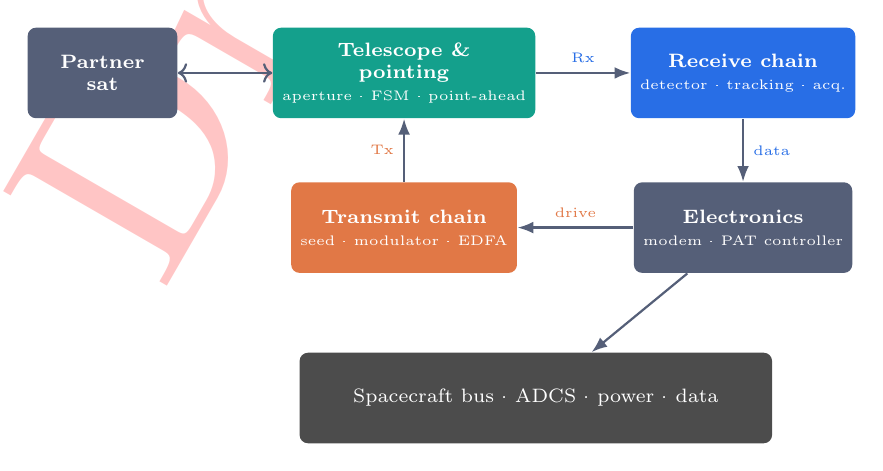
\begin{tikzpicture}[node distance=8mm and 12mm]
        \node[oblk, fill=islcslate, minimum width=1.9cm](sat){\textbf{Partner}\\\textbf{sat}};
        \node[oblk, fill=islcteal, right=of sat](tel){\textbf{Telescope \&}\\\textbf{pointing}\\\tiny aperture · FSM · point-ahead};
        \node[oblk, fill=islcblue, right=of tel](rx){\textbf{Receive chain}\\\tiny detector · tracking · acq.};
        \node[oblk, fill=islcorange, below=of tel](tx){\textbf{Transmit chain}\\\tiny seed · modulator · EDFA};
        \node[oblk, fill=islcslate, below=of rx](el){\textbf{Electronics}\\\tiny modem · PAT controller};
        \node[oblk, fill=black!70, minimum width=6cm, below=10mm of el.south -| tel.east](bus){\scriptsize Spacecraft bus · ADCS · power · data};

        \draw[oarr,<->](sat)--(tel);
        \draw[oarr](tel)-- node[above,font=\tiny,text=islcblue]{Rx} (rx);
        \draw[oarr](rx)-- node[right,font=\tiny,text=islcblue]{data} (el);
        \draw[oarr](el)-- node[above,font=\tiny,text=islcorange]{drive} (tx);
        \draw[oarr](tx.north)-- node[left,font=\tiny,text=islcorange]{Tx} (tel.south);
        \draw[oarr](el)--(bus);
    \end{tikzpicture}
    \end{center}
    \footnotesize Four blocks around \key{one shared aperture} that transmits watts, receives nanowatts and steers to microradians~\cite{sodnik2010optical}.
\end{frame}

\begin{frame}[allowframebreaks=1.2]{Aperture, transmit \& receive chains}
    \begin{itemize}
        \ai \hi{Aperture \& telescope.} A single aperture is shared by Tx and Rx to save mass; the hard part is \key{Tx/Rx isolation} --- $\sim$1\,W out vs.\ $\sim$10\,nW in is an 80--100\,dB dynamic range, won by wavelength offset (e.g.\ 1537/1563\,nm), polarization, or time-division.
    \end{itemize}
    \framebreak
    \textbf{Transmit chain} --- a fiber-laser (MOPA) stack:
    \begin{center}
    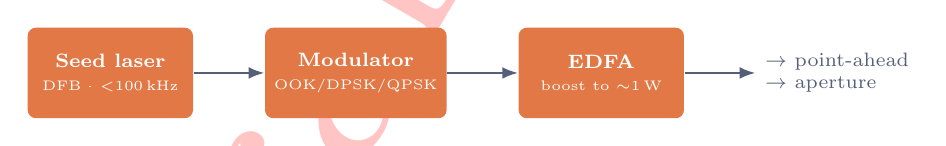
\begin{tikzpicture}[node distance=5mm and 9mm]
        \node[oblk, fill=islcorange, minimum width=2.1cm](seed){\textbf{Seed laser}\\\tiny DFB · $<$100\,kHz};
        \node[oblk, fill=islcorange, minimum width=2.1cm, right=of seed](mod){\textbf{Modulator}\\\tiny OOK/DPSK/QPSK};
        \node[oblk, fill=islcorange, minimum width=2.1cm, right=of mod](edfa){\textbf{EDFA}\\\tiny boost to $\sim$1\,W};
        \node[right=of edfa, font=\scriptsize, align=left, text=islcslate](out){$\rightarrow$ point-ahead\\$\rightarrow$ aperture};
        \draw[oarr](seed)--(mod);\draw[oarr](mod)--(edfa);\draw[oarr](edfa)--(out);
    \end{tikzpicture}
    \end{center}
    \framebreak
    \textbf{Receive chain} --- the incoming beam is tapped three ways:
    \begin{center}
    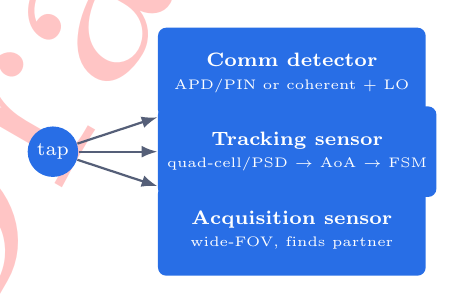
\begin{tikzpicture}[node distance=4mm and 10mm]
        \node[circle,fill=islcblue,text=white,font=\scriptsize,inner sep=2pt](tap){tap};
        \node[oblk, fill=islcblue, right=of tap, yshift=10mm, minimum width=3.4cm](comm){\textbf{Comm detector}\\\tiny APD/PIN or coherent + LO};
        \node[oblk, fill=islcblue, right=of tap, minimum width=3.4cm](trk){\textbf{Tracking sensor}\\\tiny quad-cell/PSD $\to$ AoA $\to$ FSM};
        \node[oblk, fill=islcblue, right=of tap, yshift=-10mm, minimum width=3.4cm](acq){\textbf{Acquisition sensor}\\\tiny wide-FOV, finds partner};
        \draw[oarr](tap)--(comm);\draw[oarr](tap)--(trk);\draw[oarr](tap)--(acq);
    \end{tikzpicture}
    \end{center}
    \framebreak
    \begin{itemize}
        \ai \hi{Electronics \& control.} The \key{modem} runs FEC (LDPC), framing and an ARQ retransmit layer for error-free delivery through fades; the \key{PAT controller} runs the nested acquisition/tracking loops, computes point-ahead and closes the FSM loop.
        \ai It also handles \key{Doppler}: at 1550\,nm a 15\,km/s closing rate shifts the carrier by $\sim$10\,GHz, tracked by an AFC loop on coherent systems.
    \end{itemize}
\end{frame}

%===============================================================================================
\section{Optical Components}

\begin{frame}[allowframebreaks=1.2]{Laser source \& modulation}
    \begin{columns}[T]
    \column{0.52\textwidth}
        \textbf{MOPA laser source}
        \begin{itemize}\footnotesize
            \si $\lambda = 1550$\,nm (eye-safe, EDFA band)
            \si DFB seed, linewidth $<100$\,kHz
            \si 10--40\,mW seed $\to$ 0.5--5\,W via EDFA
            \si Linear polarization (MZM requirement)
            \si RIN $< -150$\,dB/Hz; rad-hard Er-fiber
        \end{itemize}
    \column{0.48\textwidth}
        \textbf{Modulation formats}~\cite{caplan2007laser}
        \begin{itemize}\footnotesize
            \si \key{OOK}: simple, $\sim-28$\,dBm @ 10G
            \si \key{DPSK}: +3\,dB, $\sim-31$\,dBm @ 10G
            \si \key{QPSK}: coherent, $\sim-35$\,dBm @ 10G
        \end{itemize}
    \end{columns}
    \vspace{2mm}
    \begin{block}{Doppler challenge @ 1550\,nm}
    Two LEO satellites at 7.5\,km/s $\Rightarrow$ $\Delta f = f\,v/c \approx 5$\,GHz Doppler shift $\Rightarrow$ requires optical pre-compensation / AFC in the PAT loop.
    \end{block}
\end{frame}

\begin{frame}[allowframebreaks=1.2]{Beam expander, FSM \& detector}
    \begin{columns}[T]
    \column{0.5\textwidth}
        \textbf{Beam expander (Tx telescope)}
        \begin{itemize}\footnotesize
            \si Galilean afocal (no focus $\to$ no air breakdown)
            \si $D = 30$--80\,mm; CubeSat $\sim$50\,mm
            \si $\theta \approx \lambda/(\pi w_0)\approx40\,\mu$rad @ 50\,mm
            \si $\sim$20\,m footprint @ 500\,km (vs.\ 4\,km Ka)
            \si Strehl $>0.8 \Rightarrow$ WFE $<\lambda/14=111$\,nm RMS
        \end{itemize}
    \column{0.5\textwidth}
        \textbf{Fine steering mirror (FSM)}
        \begin{itemize}\footnotesize
            \si 15--30\,mm clear aperture, PZT or VCA
            \si Range $\pm1$--5\,mrad, resolution $<1\,\mu$rad
            \si Bandwidth $>500$\,Hz to reject RW harmonics
            \si Shared by Tx pointing \& PAT correction
        \end{itemize}
    \end{columns}
    \framebreak
    \begin{block}{Photodetectors}
    \footnotesize
    \key{InGaAs APD} (workhorse, LEO--LEO): gain $M=5$--20, $-30$ to $-35$\,dBm @ 10G, room temperature, 900--1650\,nm. \quad
    \key{SNSPD} (deep-space, photon-starved): single-photon, $>$90\% efficiency, $<$50\,ps jitter --- flown on NASA LLCD~\cite{boroson2014llcd}.
    \end{block}
    \begin{center}\scriptsize
    
\begin{tikzpicture}[node distance=3mm and 6mm]
        \node[oblk,fill=islcteal,minimum width=1.7cm](t){\textbf{Cassegrain}\\\tiny 50--100\,mm};
        \node[oblk,fill=islcteal,minimum width=1.7cm,right=of t](f){\textbf{BPF}\\\tiny 0.3--1\,nm};
        \node[oblk,fill=islcteal,minimum width=1.7cm,right=of f](fo){\textbf{Focus}\\\tiny f/4--f/8};
        \node[oblk,fill=islcteal,minimum width=1.7cm,right=of fo](apd){\textbf{APD}\\\tiny $M{=}10$--15};
        \node[oblk,fill=islcteal,minimum width=1.7cm,right=of apd](dsp){\textbf{TIA+DSP}\\\tiny demod·FEC};
        \draw[oarr](t)--(f);\draw[oarr](f)--(fo);\draw[oarr](fo)--(apd);\draw[oarr](apd)--(dsp);
    \end{tikzpicture}
    \end{center}
    \centering\footnotesize Complete receive chain. \quad Key coupling: $\theta\propto\lambda/D$ --- larger aperture $=$ narrower beam $=$ higher gain $=$ tighter pointing requirement.
\end{frame}

%===============================================================================================
\section{Pointing, Acquisition \& Tracking}

\begin{frame}[allowframebreaks=1.2]{Point-ahead \& acquisition}
    \begin{itemize}
        \ai Light takes time to cross the link and both satellites move --- you transmit toward where the partner \key{WILL be} while its beam arrives from where it \key{WAS}~\cite{kaushal2017optical}.
        \ai The lead angle is
        \begin{equation*}
            \alpha_{PA}\approx \frac{2v_\perp}{c}.
        \end{equation*}
        \si Cross-plane LEO: $v_\perp$ up to $\sim$15\,km/s gives $\sim$100\,$\mu$rad --- comparable to the whole beamwidth, so a dedicated actuator is required.
        \si Same-plane crosslinks move together: point-ahead nearly vanishes.
    \end{itemize}
    \framebreak
    \textbf{From blind to locked --- 3-stage PAT}
    \begin{center}
    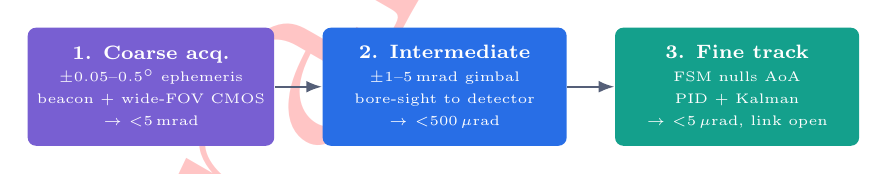
\begin{tikzpicture}[node distance=6mm]
        \node[oblk,fill=islcpurple,minimum width=3.1cm,minimum height=1.5cm](s1){\textbf{1. Coarse acq.}\\\tiny $\pm0.05$--$0.5^\circ$ ephemeris\\\tiny beacon + wide-FOV CMOS\\\tiny $\to$ $<$5\,mrad};
        \node[oblk,fill=islcblue,minimum width=3.1cm,minimum height=1.5cm,right=of s1](s2){\textbf{2. Intermediate}\\\tiny $\pm1$--5\,mrad gimbal\\\tiny bore-sight to detector\\\tiny $\to$ $<$500\,$\mu$rad};
        \node[oblk,fill=islcteal,minimum width=3.1cm,minimum height=1.5cm,right=of s2](s3){\textbf{3. Fine track}\\\tiny FSM nulls AoA\\\tiny PID + Kalman\\\tiny $\to$ $<$5\,$\mu$rad, link open};
        \draw[oarr](s1)--(s2);\draw[oarr](s2)--(s3);
    \end{tikzpicture}
    \end{center}
\end{frame}

\begin{frame}[allowframebreaks=1.2]{FSM tracking-loop design}
    \begin{itemize}
        \ai \hi{Plant} --- a lightly damped resonant mirror:
        \begin{equation*}
            P(s)=\frac{K_{act}\,\omega_n^{2}}{s^{2}+2\zeta\omega_n s+\omega_n^{2}},\quad
            \begin{aligned}
            &\omega_n = 2\pi\!\times\!500\text{--}2000\ \text{rad/s}\\
            &\zeta = 0.01\text{--}0.05,\ K_{act}=10\text{--}50\,\mu\text{rad/V}
            \end{aligned}
        \end{equation*}
        \ai \hi{Controller} $C(s)=$ PID $\times$ notches, crossover $f_c\approx300$\,Hz, phase margin $\ge45^\circ$, gain margin $\ge6$\,dB. The notch
        \begin{equation*}
            N(s)=\frac{s^{2}+2\zeta_z\omega_n s+\omega_n^{2}}{s^{2}+2\zeta_p\omega_n s+\omega_n^{2}},\quad \zeta_z\!=\!0.001,\ \zeta_p\!=\!0.3\text{--}0.5
        \end{equation*}
        places a deep null at each mechanical / reaction-wheel resonance.
    \end{itemize}
    \framebreak
    \begin{itemize}
        \ai \hi{Sensing.} 4-quadrant detector (up to 100\,kHz, $\pm$20\% spot linear range) gives the centroid error
        \begin{equation*}
            \varepsilon_x=\frac{(A+B)-(C+D)}{A+B+C+D}.
        \end{equation*}
        \ai \hi{Kalman estimator.} State $x=[\theta,\dot\theta,d_{dist}]^\mathsf{T}$ with update
        \begin{equation*}
            K_k = P_k^{-}H^\mathsf{T}\!\left(HP_k^{-}H^\mathsf{T}+R\right)^{-1},\quad R\approx(0.5\,\mu\text{rad})^2 .
        \end{equation*}
        \si Disturbance feed-forward $u_{ff}=-K_{ff}\hat d$ cancels reaction-wheel harmonics by \key{15--25\,dB} vs.\ PID alone.
    \end{itemize}
\end{frame}

%===============================================================================================
\section{Wavefront Error Budget}

\begin{frame}[allowframebreaks=1.2]{From surface to Strehl}
    \begin{itemize}
        \ai Wavefront quality maps to coupling efficiency through the \key{Mar\'echal approximation}~\cite{born1999principles}:
        \begin{equation*}
            \tcbhighmath[boxrule=1pt,arc=2pt,colback=islcteal!4,colframe=islcorange]{%
            S \approx \exp\!\left[-\left(\frac{2\pi\sigma}{\lambda}\right)^{2}\right]}
        \end{equation*}
        where $\sigma$ is the RMS wavefront error. Diffraction-limited $\equiv S>0.8$.
    \end{itemize}
    \framebreak
    \begin{block}{Representative WFE budget (RSS)}
    \centering\scriptsize
    \begin{tabular}{l r}
        \hline
        \textbf{Contributor} & \textbf{nm RMS}\\
        \hline
        Primary mirror surface figure & 11\\
        Secondary mirror figure       & 8\\
        Relay lens transmitted WFE    & 6\\
        AR/HR coating micro-roughness & 4\\
        Mirror decenter (assembly)    & 9\\
        Axial despace / focus error   & 7\\
        Thermal gradient deformation  & 12\\
        Mounting stress (flexures)    & 6\\
        Residual vibration post-FSM   & 4\\
        \hline
        \textbf{RSS total} & \textbf{23.7}\\
        \hline
    \end{tabular}
    \end{block}
    \centering Strehl $S\approx0.91 \Rightarrow$ \key{diffraction-limited} (criterion $S>0.8$).
    \framebreak
    \textbf{WFE design process --- requirement to hardware}
    \begin{enumerate}[label=\arabic*.]\footnotesize
        \item System Strehl requirement (from link budget); set target to 70\% of limit for margin.
        \item Zemax sensitivity analysis: $S_{ij}=\partial\text{WFE}_i/\partial\text{DOF}_j$ identifies dominant terms (e.g.\ secondary decenter $\to$ coma).
        \item WFE allocation: invert sensitivities, $\delta_j=\sigma_i/S_{ij}$, iterate to achievable tolerances.
        \item Manufacture \& metrology: Fizeau interferometry ($\lambda/50$), ion-beam polishing.
        \item Space qualification: TVAC, vibration, shock, TID.
        \item End-to-end link test with range-equivalent attenuation.
    \end{enumerate}
\end{frame}

%===============================================================================================
\section{CubeSat Link Budget}

\begin{frame}[allowframebreaks=1.2]{CubeSat OISL trade-space}
    \begin{equation*}
        P_{rx}=P_{tx}\,\eta_{tx}\frac{\pi D_{tx}^{2}}{4\lambda^{2}}\cdot\frac{\pi D_{rx}^{2}}{4R^{2}}\,\eta_{rx}\,L_{point}
    \end{equation*}
    \begin{columns}[T]
    \column{0.55\textwidth}
    \scriptsize
    \begin{tabular}{l r}
        \hline
        \textbf{Term (D=40\,mm, 500\,km)} & \textbf{dB}\\
        \hline
        Tx power (0.5\,W)        & $+27.0$\,dBm\\
        Tx optical eff.\ $\eta_{tx}=0.75$ & $-1.2$\\
        Tx aperture gain         & $+76.8$\\
        Free-space path loss     & $-278.2$\\
        Rx aperture (eff.\ area)  & $+67.2$\\
        Rx optical eff.\ $\eta_{rx}=0.60$ & $-2.2$\\
        Pointing loss            & $-2.0$\\
        \hline
        \textbf{Received power}  & $\mathbf{-112.6}$\,\textbf{dBm}\\
        \hline
    \end{tabular}
    \column{0.45\textwidth}
        \begin{itemize}\footnotesize
            \ai APD sensitivity @ 1\,Gbps: \hi{$-41$\,dBm}
            \ai Link margin: \hi{$+28$\,dB}
            \ai Max data rate at these params: \hi{$\sim$3\,Gbps}
        \end{itemize}
    \end{columns}
    \framebreak
    \begin{block}{The two scaling laws that govern everything}
    \footnotesize
    \key{$P_{rx}\propto D^{4}$} --- both apertures scale received power; doubling $D$ on both sides $=+12$\,dB ($\times16$). \\
    \key{$P_{rx}\propto 1/R^{2}$} --- doubling range costs 6\,dB.
    \end{block}
    \begin{itemize}\footnotesize
        \ai \hi{CubeSat limit:} 1U constrains aperture to $\sim$40--50\,mm $\Rightarrow$ Gbps+ links practical to $<$800\,km with 0.5\,W Tx.
        \ai \hi{Power tradeoff:} an EDFA at 1\,W optical draws $\sim$5--8\,W DC --- 50--80\% of a 10\,W CubeSat budget, the dominant system constraint.
    \end{itemize}
\end{frame}

%===============================================================================================
\section{Experimental Test Setup}

\begin{frame}{Experimental strategy \& test hierarchy}
    \begin{columns}[T]
    \column{0.5\textwidth}
        \begin{itemize}\footnotesize
            \ai \key{Component-level}: characterize each optical element (laser, FSM, detector, telescope) in isolation.
            \ai \key{Subsystem-level}: validate Tx chain, Rx chain and PAT loop independently.
            \ai \key{System-level}: end-to-end link with range-equivalent path loss.
            \ai \key{Environmental}: TVAC, vibration, radiation per ECSS / NASA.
        \end{itemize}
    \column{0.5\textwidth}
        \scriptsize
        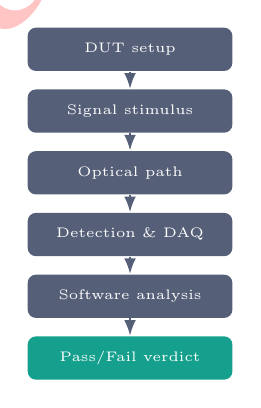
\begin{tikzpicture}[node distance=2.2mm, every node/.style={oblk,fill=islcslate,minimum width=2.6cm,minimum height=0.55cm,font=\tiny}]
            \node(a){DUT setup};
            \node[below=of a](b){Signal stimulus};
            \node[below=of b](c){Optical path};
            \node[below=of c](d){Detection \& DAQ};
            \node[below=of d](e){Software analysis};
            \node[below=of e,fill=islcteal](f){Pass/Fail verdict};
            \draw[oarr](a)--(b);\draw[oarr](b)--(c);\draw[oarr](c)--(d);\draw[oarr](d)--(e);\draw[oarr](e)--(f);
        \end{tikzpicture}
    \end{columns}
\end{frame}

\begin{frame}[allowframebreaks=1.2]{Hardware: bench, Tx \& Rx instruments}
    \textbf{Optical bench}
    \begin{itemize}\footnotesize
        \si Active-pneumatic isolation table (Newport RS2000/TMC); 6-DOF kinematic mounts (sub-$\mu$rad).
        \si 2-axis piezo mirror (PI S-330) emulates jitter; Galilean beam expander; PBS + waveplates.
        \si \key{Fizeau interferometer} ($\lambda/100$), \key{Shack--Hartmann WFS} (150 lenslets), beam profiler ($M^2$), calibrated power meter + ND set; SMF-28 delay-line emulator.
    \end{itemize}
    \framebreak
    \textbf{Tx-chain instruments}
    \begin{itemize}\footnotesize
        \si Tunable laser source (Keysight 81600B / Santec TSL-710), 1480--1640\,nm, $<$100\,kHz.
        \si Optical spectrum analyzer (Yokogawa AQ6370D), 0.02\,nm res, $>$70\,dB --- OSNR/ASE.
        \si VNA (Keysight E5063A) for MZM EO bandwidth ($>$40\,GHz); AWG (Keysight M8195A) PRBS-31 / IQ drive.
    \end{itemize}
    \framebreak
    \textbf{Rx-chain instruments}
    \begin{itemize}\footnotesize
        \si APD characterization: Keithley 2400 SMU bias, responsivity, $-3$\,dB BW, NEP (FEMTO TIA + SR830).
        \si \key{BER \& sensitivity}: BERT (Anritsu MP1800A), VOA sweep ($-25$ to $-55$\,dBm), CDR, 80\,GHz sampling scope --- read sensitivity at BER $=10^{-12}$.
    \end{itemize}
\end{frame}

\begin{frame}[allowframebreaks=1.2]{PAT test, DAQ/FPGA \& software stack}
    \textbf{PAT test hardware}
    \begin{itemize}\footnotesize
        \si Jitter emulator (PI S-330.2SL + AWG, 0--2\,mrad, 1--1000\,Hz); 4-QD (Hamamatsu G6849, $>$100\,kHz).
        \si FSM + E-727 driver ($\pm10$\,V $\to\pm5$\,mrad, $<$0.1\,$\mu$rad); coarse gimbal; CMOS InGaAs camera.
        \si \key{Real-time controller}: NI cRIO-9049 (Xilinx Kintex-7) running PID + notch + Kalman at 50--100\,kHz.
    \end{itemize}
    \framebreak
    \textbf{FPGA control loop (100\,kHz, $\sim$10\,$\mu$s budget)}
    \begin{enumerate}[label=\arabic*.]\scriptsize
        \item ADC read 4-QD $\to$ centroid error (10\,$\mu$s)
        \item Bandpass error filter, 100--800\,Hz (1\,$\mu$s)
        \item Velocity-form PID (2\,$\mu$s)
        \item IIR notch sections at $\omega_n$, $f_{RW}$, $2f_{RW}$, $3f_{RW}$ (2\,$\mu$s)
        \item Kalman predict + disturbance feed-forward (3\,$\mu$s)
        \item DAC write to FSM, saturated at $\pm9.5$\,V (2\,$\mu$s)
    \end{enumerate}
    \framebreak
    \textbf{Software layers}
    \begin{itemize}\footnotesize
        \si L5 Analysis: Python/MATLAB --- NumPy, SciPy, matplotlib, pandas.
        \si L4 Orchestration: LabVIEW TestStand / pytest, SCPI drivers, CI.
        \si L3 Real-time: LabVIEW RT / Simulink RT --- PAT state machine, Kalman.
        \si L2 FPGA: VHDL/Vivado --- PID + notch, 100\,kHz.
        \si L1 Drivers: NI-VISA / NI-DAQmx, SCPI over GPIB/USB/LAN.
    \end{itemize}
\end{frame}

\begin{frame}{Integrated hardware + software test chain}
    \begin{center}
    \scriptsize
    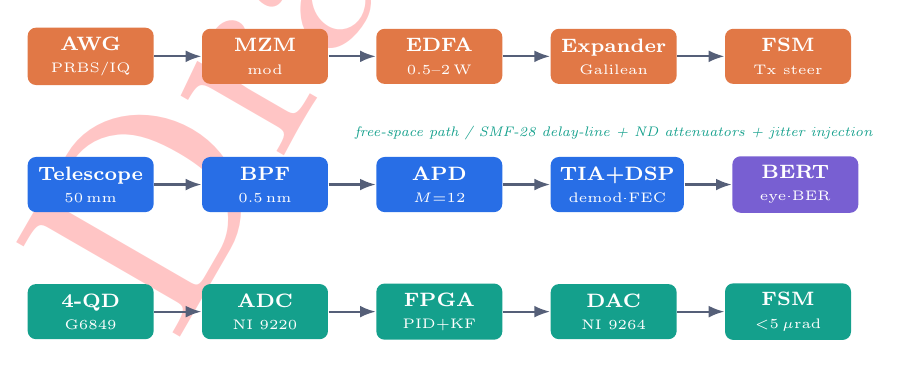
\begin{tikzpicture}[node distance=2.5mm and 6mm]
        % Tx row
        \node[oblk,fill=islcorange,minimum width=1.6cm,minimum height=0.7cm](awg){\textbf{AWG}\\\tiny PRBS/IQ};
        \node[oblk,fill=islcorange,minimum width=1.6cm,minimum height=0.7cm,right=of awg](mzm){\textbf{MZM}\\\tiny mod};
        \node[oblk,fill=islcorange,minimum width=1.6cm,minimum height=0.7cm,right=of mzm](edfa){\textbf{EDFA}\\\tiny 0.5--2\,W};
        \node[oblk,fill=islcorange,minimum width=1.6cm,minimum height=0.7cm,right=of edfa](be){\textbf{Expander}\\\tiny Galilean};
        \node[oblk,fill=islcorange,minimum width=1.6cm,minimum height=0.7cm,right=of be](fsm1){\textbf{FSM}\\\tiny Tx steer};
        \draw[oarr](awg)--(mzm);\draw[oarr](mzm)--(edfa);\draw[oarr](edfa)--(be);\draw[oarr](be)--(fsm1);
        % channel
        \node[below=4mm of be, text=islcteal, font=\tiny\itshape](ch){free-space path / SMF-28 delay-line + ND attenuators + jitter injection};
        % Rx row
        \node[oblk,fill=islcblue,minimum width=1.6cm,minimum height=0.7cm,below=9mm of awg](tele){\textbf{Telescope}\\\tiny 50\,mm};
        \node[oblk,fill=islcblue,minimum width=1.6cm,minimum height=0.7cm,right=of tele](bpf){\textbf{BPF}\\\tiny 0.5\,nm};
        \node[oblk,fill=islcblue,minimum width=1.6cm,minimum height=0.7cm,right=of bpf](apd){\textbf{APD}\\\tiny $M{=}12$};
        \node[oblk,fill=islcblue,minimum width=1.6cm,minimum height=0.7cm,right=of apd](tia){\textbf{TIA+DSP}\\\tiny demod·FEC};
        \node[oblk,fill=islcpurple,minimum width=1.6cm,minimum height=0.7cm,right=of tia](bert){\textbf{BERT}\\\tiny eye·BER};
        \draw[oarr](tele)--(bpf);\draw[oarr](bpf)--(apd);\draw[oarr](apd)--(tia);\draw[oarr](tia)--(bert);
        % PAT row
        \node[oblk,fill=islcteal,minimum width=1.6cm,minimum height=0.7cm,below=9mm of tele](qd){\textbf{4-QD}\\\tiny G6849};
        \node[oblk,fill=islcteal,minimum width=1.6cm,minimum height=0.7cm,right=of qd](adc){\textbf{ADC}\\\tiny NI 9220};
        \node[oblk,fill=islcteal,minimum width=1.6cm,minimum height=0.7cm,right=of adc](fpga){\textbf{FPGA}\\\tiny PID+KF};
        \node[oblk,fill=islcteal,minimum width=1.6cm,minimum height=0.7cm,right=of fpga](dac){\textbf{DAC}\\\tiny NI 9264};
        \node[oblk,fill=islcteal,minimum width=1.6cm,minimum height=0.7cm,right=of dac](fsm2){\textbf{FSM}\\\tiny $<$5\,$\mu$rad};
        \draw[oarr](qd)--(adc);\draw[oarr](adc)--(fpga);\draw[oarr](fpga)--(dac);\draw[oarr](dac)--(fsm2);
    \end{tikzpicture}
    \end{center}
    \footnotesize Top: transmit side. Middle: emulated channel. Bottom: closed PAT tracking loop.
\end{frame}

\begin{frame}{Key measurement sequences \& acceptance criteria}
    \footnotesize
    \begin{columns}[T]
    \column{0.33\textwidth}
        \textbf{WFE \& Strehl}
        \begin{itemize}\scriptsize
            \si SH-WFS, 100 frames, Zernike Z4--Z37
            \si RSS WFE; Strehl via Mar\'echal
        \end{itemize}
        \textcolor{islcteal}{$\checkmark$ RSS WFE $<$30\,nm, $S>0.80$}
    \column{0.33\textwidth}
        \textbf{FSM loop closure}
        \begin{itemize}\scriptsize
            \si Swept-sine $\to$ $H(f)$, fit $\omega_n,\zeta$
            \si PID+notch, inject 60/120/180\,Hz
        \end{itemize}
        \textcolor{islcteal}{$\checkmark$ RMS $<$5\,$\mu$rad, BW $>$500\,Hz}
    \column{0.33\textwidth}
        \textbf{BER waterfall}
        \begin{itemize}\scriptsize
            \si Sweep VOA, fit $0.5\,\mathrm{erfc}(Q/\sqrt2)$
            \si Margin $\ge3$\,dB
        \end{itemize}
        \textcolor{islcteal}{$\checkmark$ $\le-35$\,dBm @ 10G, $10^{-12}$}
    \end{columns}
    \vspace{2mm}
    \begin{block}{Environmental qualification}
    \scriptsize TVAC ($<10^{-6}$\,mbar, $-40$ to $+70^\circ$C, in-situ WFS) --- WFE RSS $<$35\,nm, $S>0.78$. \quad
    Vibration (GEVS-7000A, 14.1\,$g_{rms}$) + 3000\,g shock. \quad Co-60 TID (10--50\,krad Si) on EDFA fiber \& APD.
    \end{block}
\end{frame}

%===============================================================================================
\section{Flown Hardware \& Conclusion}

\begin{frame}{Reference CubeSat-class terminals}
    \begin{columns}[T]
    \column{0.5\textwidth}
        \begin{block}{CLICK-B/C~\cite{cahoy2020click}}
        \footnotesize MIT / UF / NASA
        \begin{itemize}\scriptsize
            \si Two 3U CubeSats; sub-2U terminals
            \si 20\,Mbps full-duplex, 25--580\,km
            \si 1537/1563\,nm, $\sim$200\,mW, direct detection
            \si MEMS fast-steering mirror \& ranging
        \end{itemize}
        \end{block}
    \column{0.5\textwidth}
        \begin{block}{TBIRD~\cite{robinson2018tbird,schieler2023tbird}}
        \footnotesize MIT Lincoln Laboratory
        \begin{itemize}\scriptsize
            \si 3U payload on a 6U bus
            \si 100 / 200\,Gbps downlink to ground
            \si Coherent fiber-coupled COTS transceivers
            \si ARQ error-free delivery --- up to 4.8\,TB/pass
        \end{itemize}
        \end{block}
    \end{columns}
    \vspace{2mm}
    \centering\footnotesize Interoperability is converging on the SDA \key{Optical Communications Terminal (OCT)} standard~\cite{sda2022oct}.
\end{frame}

\begin{frame}{Key takeaways}
    \begin{itemize}
        \ai OISL is the \key{laser backbone} of modern constellations --- vast gain and bandwidth from a tiny aperture~\cite{kaushal2017optical,toyoshima2021trends}.
        \ai The narrow beam makes \hi{pointing, not photons,} the dominant engineering risk.
        \ai The link budget governs everything: \key{$P_{rx}\propto D^{4}$} --- aperture is the highest-leverage variable.
        \ai Point-ahead, Tx/Rx isolation and FSM jitter rejection are the defining sub-problems; the \key{FSM tracking loop} (PID + notch, $>$500\,Hz, Kalman) is the critical control subsystem.
        \ai CubeSat-scale OISL ($<$50\,mm, $<$1\,W, 1U) enables \key{Gbps+ at $<$800\,km} --- feasible today. Frontiers: MEMS FSM, photonic-IC transceivers, coherent QPSK.
    \end{itemize}
\end{frame}

%-----------------------------------------------------------------------------------------------
\begin{frame}{}
    \centering
    \vfill
    {\fontsize{22}{26}\selectfont \textcolor{islcteal}{\textbf{Thank you}}}\\[4mm]
    {\large Questions \& discussion}
    \vfill
\end{frame}
%-----------------------------------------------------------------------------------------------
\begin{frame}[allowframebreaks=0.9]{References}
    \bibliographystyle{model1-num-names}
    \bibliography{cas-refs}
    \framebreak
\end{frame}
%-----------------------------------------------------------------------------------------------
\end{document}



% These "\usepackage{}" commands import packages into the LaTeX document.
\usepackage[english]{babel}
\usepackage[light,math]{anttor}
\usepackage{graphicx,graphbox}
\usepackage{parskip}
\usepackage{amsmath}
\usepackage{caption}
\usepackage{subcaption}
\usepackage{background}
\usepackage{xcolor}

\usepackage[skins, theorems]{tcolorbox}
\usepackage{pifont}
\usepackage{amssymb,enumitem}
\usepackage{indentfirst}
\usepackage{tabularray}
\usepackage{hyperref}
\usepackage{cleveref}
\usepackage{array}
\usepackage{multirow}
\setbeamertemplate{caption}[numbered]
\usepackage[square,numbers,sort&compress]{natbib}
\renewcommand{\bibsection}{\subsubsection*{\bibname}}
\setbeamertemplate{frametitle continuation}[from second][(contd.)]
\usepackage{setspace}
\onehalfspacing

% Extra TikZ libraries for the block diagrams (tikz + positioning come from the class)
\usetikzlibrary{arrows.meta,positioning,shapes.geometric,fit,backgrounds,calc}

\usetheme{Madrid}
\usecolortheme{default}
\hypersetup{
    colorlinks=true,
    linkcolor=cyan,
    urlcolor=cyan,
    citecolor=cyan,
}

%------------------------------------------------------------
% ISLC colour palette (complements the kaist-* colours from the class)
\definecolor{islcteal}{RGB}{20,160,140}
\definecolor{islcblue}{RGB}{40,110,230}
\definecolor{islcorange}{RGB}{225,120,70}
\definecolor{islcslate}{RGB}{85,95,120}
\definecolor{islcpurple}{RGB}{120,95,210}

% Shorthand bullets and highlight macros to keep the body readable
\newcommand{\ai}{\item[\textcolor{islcteal}{\ding{228}}]}      % primary bullet
\newcommand{\si}{\item[\textcolor{islcorange}{\ding{167}}]}    % sub bullet
\newcommand{\hi}[1]{\textcolor{islcorange}{\textbf{#1}}}       % inline highlight
\newcommand{\key}[1]{\textcolor{islcblue}{\textbf{#1}}}        % inline key term

% Generic TikZ block styles for the architecture / chain diagrams
\tikzset{
  oblk/.style={rectangle, rounded corners=3pt, draw=none, text=white,
               align=center, font=\scriptsize, minimum width=2.6cm, minimum height=1.15cm},
  oarr/.style={-{Latex[length=2mm]}, thick, islcslate},
}

%------------------------------------------------------------
% Title-page information
\title[ISLC for CubeSats] %optional
{Inter-Satellite Laser Communication for CubeSat Platforms}

\subtitle{Optical terminal architecture, design \& experimental setup}

\author[Dinaol Gadisa] % (optional)
{Dinaol Gadisa\inst{1} \and Hyochoong Bang\inst{1}}

\institute[ASCL] % (optional)
{
  \inst{1}%
  Aerospace System and Control Lab, Department of Aerospace Engineering, KAIST\\
}

\date[ASCL-P2026] % (optional)
{ISLC research report, June 2026}

%End of title-page configuration block
%------------------------------------------------------------

% Put a table of contents at the start of every section
\AtBeginSection[]
{
  \begin{frame}
    \frametitle{Table of Contents}
    \tableofcontents[currentsection]
  \end{frame}
}

\renewcommand{\titlelogo}{logo/ascl logo.svg}
\renewcommand{\slidelogo}{logo/ascl logo.svg}
% If \includesvg is unavailable, drop the extension and use a raster logo instead:
% \renewcommand{\titlelogo}{logo/ascl logo}
% \renewcommand{\slidelogo}{logo/ascl logo}

\backgroundsetup{
  scale=0.6,
  angle=0,
  opacity=0.02,
  contents={
    
\includegraphics[width=\textwidth,height=\textwidth]{figs/download.png}}
}

\renewcommand{\slidefoot}{Dinaol Gadisa}
%-----------------------------------------------------------------------------------------------
\begin{document}

\frame{\titlepage}

%===============================================================================================
\section{Introduction \& Motivation}

\begin{frame}[t,allowframebreaks=1.2]{Why optical inter-satellite links?}
    \begin{itemize}
        \ai Inter-satellite laser communication (\hi{ISLC}, also \hi{OISL}) links satellites \key{directly} to one another with laser beams instead of routing every bit down to the ground and back up~\cite{kaushal2017optical,sodnik2010optical}.
        \ai The carrier is a near-infrared laser --- typically \key{1550\,nm} ($\sim$193\,THz) --- inherited from the fiber-telecom ecosystem.
        \ai Chained across a constellation, the links form a \key{low-latency optical mesh} that moves data in orbit --- the in-space backbone of Starlink, Kuiper and the SDA transport layer~\cite{chaudhry2021free,sda2022oct}.
    \end{itemize}
    \framebreak
    \begin{block}{Optical vs.\ RF --- why lasers win in space~\cite{kaushal2017optical}}
    \centering\footnotesize
    \begin{tabular}{l l l}
        \hline
        \textbf{Parameter} & \textbf{Ka-band RF} & \textbf{OISL @ 1550\,nm}\\
        \hline
        Data rate      & 100--600\,Mbps   & 1--100\,Gbps\\
        Carrier        & 26--40\,GHz      & $\sim$193\,THz\\
        Beam divergence& $\sim0.5$--$2^\circ$ & $\sim$10--100\,$\mu$rad\\
        Aperture       & 200--600\,mm     & 30--100\,mm\\
        Licensing      & \textcolor{red}{Required} & \textcolor{islcteal}{None (LPI/LPD)}\\
        \hline
    \end{tabular}
    \end{block}
    \begin{itemize}
        \ai \hi{The catch:} a tens-of-$\mu$rad beam must be pointed to a few $\mu$rad across thousands of km --- \key{pointing, not photons, is the hard problem}.
    \end{itemize}
\end{frame}

\begin{frame}{Advantages of OISL}
    \begin{columns}[T]
    \column{0.5\textwidth}
        \begin{itemize}
            \ai \hi{10--100$\times$} higher data rate than Ka-band RF
            \ai \hi{$\sim$10\,$\mu$rad} beam divergence (vs.\ $\sim1^\circ$ for RF)
            \ai \hi{No ITU} frequency licensing required
            \ai \hi{$<$50\%} mass \& aperture vs.\ equivalent RF
        \end{itemize}
    \column{0.5\textwidth}
        \begin{block}{CubeSat relevance~\cite{toyoshima2021trends,cahoy2020click}}
        A 50\,mm-aperture OISL achieves \key{Gbps at 500\,km} in a $\sim$0.5U volume --- impossible with RF in the same form factor.
        \end{block}
    \end{columns}
\end{frame}

%===============================================================================================
\section{Link Fundamentals}

\begin{frame}[allowframebreaks=1.2]{The link in one equation}
    \begin{itemize}
        \ai The received power follows the free-space optical link equation~\cite{hemmati2009near,caplan2007laser}:
    \end{itemize}
    \begin{equation*}
        \tcbhighmath[boxrule=1pt,arc=2pt,colback=islcteal!4,colframe=islcblue,drop fuzzy shadow=islcslate]{%
        P_{rx} = P_{tx}\, G_{tx}\, \left(\frac{\lambda}{4\pi R}\right)^{2} G_{rx}\, L_{point}\, L_{impl}}
    \end{equation*}
    \begin{itemize}
        \si \hi{Aperture gain} $G = (\pi D/\lambda)^2 \approx +100$\,dB for a diffraction-limited 5\,cm telescope.
        \si \hi{Free-space loss} $(\lambda/4\pi R)^2 \approx -262$\,dB over 1500\,km at 1550\,nm.
        \si \hi{Pointing loss} $\propto e^{-2(\theta/\theta_0)^2}$ --- $\tfrac13$ of a beamwidth off $\approx$ 1\,dB lost.
    \end{itemize}
    \framebreak
    \begin{itemize}
        \ai Two competing quantities set everything: \key{antenna gain} and \key{beam divergence}
        \begin{equation*}
            G = \left(\frac{\pi D}{\lambda}\right)^{2}, \qquad \theta \approx \frac{\lambda}{D}\approx\frac{\lambda}{\pi w_0}.
        \end{equation*}
        \ai Enormous gains fight an enormous path loss; \key{sensitivity} is then set by \hi{photons/bit}:
        \begin{equation*}
            P_{req} = \left(\frac{\text{photons}}{\text{bit}}\right)\frac{hc}{\lambda}\,R_b .
        \end{equation*}
        \si OOK $\approx$ tens, DPSK $\approx 38$, coherent $\approx 9$ photons/bit at BER $10^{-9}$~\cite{caplan2007laser}.
    \end{itemize}
\end{frame}

%===============================================================================================
\section{Optical Terminal Architecture}

\begin{frame}{Terminal architecture at a glance}
    \begin{center}
    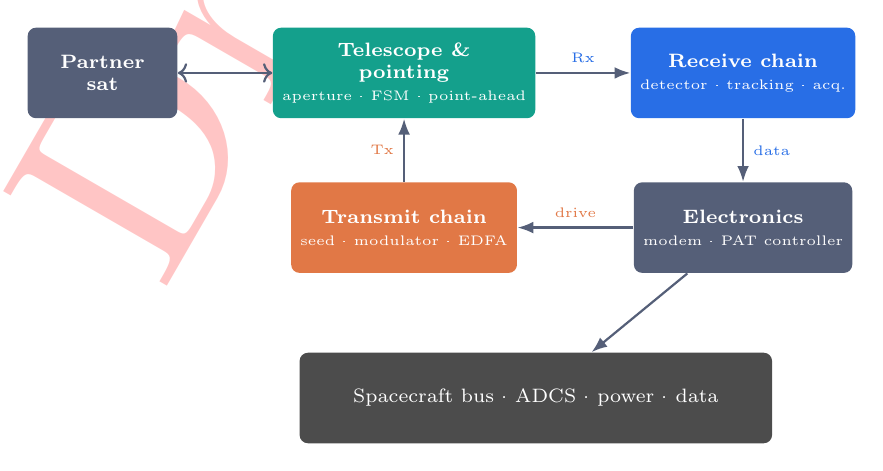
\begin{tikzpicture}[node distance=8mm and 12mm]
        \node[oblk, fill=islcslate, minimum width=1.9cm](sat){\textbf{Partner}\\\textbf{sat}};
        \node[oblk, fill=islcteal, right=of sat](tel){\textbf{Telescope \&}\\\textbf{pointing}\\\tiny aperture · FSM · point-ahead};
        \node[oblk, fill=islcblue, right=of tel](rx){\textbf{Receive chain}\\\tiny detector · tracking · acq.};
        \node[oblk, fill=islcorange, below=of tel](tx){\textbf{Transmit chain}\\\tiny seed · modulator · EDFA};
        \node[oblk, fill=islcslate, below=of rx](el){\textbf{Electronics}\\\tiny modem · PAT controller};
        \node[oblk, fill=black!70, minimum width=6cm, below=10mm of el.south -| tel.east](bus){\scriptsize Spacecraft bus · ADCS · power · data};

        \draw[oarr,<->](sat)--(tel);
        \draw[oarr](tel)-- node[above,font=\tiny,text=islcblue]{Rx} (rx);
        \draw[oarr](rx)-- node[right,font=\tiny,text=islcblue]{data} (el);
        \draw[oarr](el)-- node[above,font=\tiny,text=islcorange]{drive} (tx);
        \draw[oarr](tx.north)-- node[left,font=\tiny,text=islcorange]{Tx} (tel.south);
        \draw[oarr](el)--(bus);
    \end{tikzpicture}
    \end{center}
    \footnotesize Four blocks around \key{one shared aperture} that transmits watts, receives nanowatts and steers to microradians~\cite{sodnik2010optical}.
\end{frame}

\begin{frame}[allowframebreaks=1.2]{Aperture, transmit \& receive chains}
    \begin{itemize}
        \ai \hi{Aperture \& telescope.} A single aperture is shared by Tx and Rx to save mass; the hard part is \key{Tx/Rx isolation} --- $\sim$1\,W out vs.\ $\sim$10\,nW in is an 80--100\,dB dynamic range, won by wavelength offset (e.g.\ 1537/1563\,nm), polarization, or time-division.
    \end{itemize}
    \framebreak
    \textbf{Transmit chain} --- a fiber-laser (MOPA) stack:
    \begin{center}
    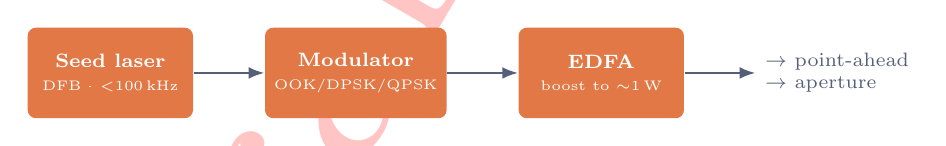
\begin{tikzpicture}[node distance=5mm and 9mm]
        \node[oblk, fill=islcorange, minimum width=2.1cm](seed){\textbf{Seed laser}\\\tiny DFB · $<$100\,kHz};
        \node[oblk, fill=islcorange, minimum width=2.1cm, right=of seed](mod){\textbf{Modulator}\\\tiny OOK/DPSK/QPSK};
        \node[oblk, fill=islcorange, minimum width=2.1cm, right=of mod](edfa){\textbf{EDFA}\\\tiny boost to $\sim$1\,W};
        \node[right=of edfa, font=\scriptsize, align=left, text=islcslate](out){$\rightarrow$ point-ahead\\$\rightarrow$ aperture};
        \draw[oarr](seed)--(mod);\draw[oarr](mod)--(edfa);\draw[oarr](edfa)--(out);
    \end{tikzpicture}
    \end{center}
    \framebreak
    \textbf{Receive chain} --- the incoming beam is tapped three ways:
    \begin{center}
    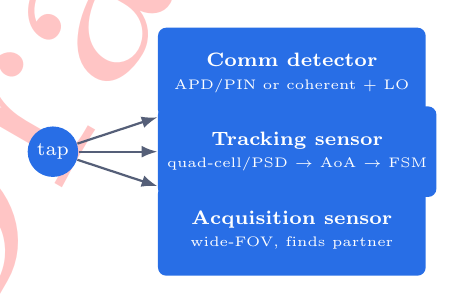
\begin{tikzpicture}[node distance=4mm and 10mm]
        \node[circle,fill=islcblue,text=white,font=\scriptsize,inner sep=2pt](tap){tap};
        \node[oblk, fill=islcblue, right=of tap, yshift=10mm, minimum width=3.4cm](comm){\textbf{Comm detector}\\\tiny APD/PIN or coherent + LO};
        \node[oblk, fill=islcblue, right=of tap, minimum width=3.4cm](trk){\textbf{Tracking sensor}\\\tiny quad-cell/PSD $\to$ AoA $\to$ FSM};
        \node[oblk, fill=islcblue, right=of tap, yshift=-10mm, minimum width=3.4cm](acq){\textbf{Acquisition sensor}\\\tiny wide-FOV, finds partner};
        \draw[oarr](tap)--(comm);\draw[oarr](tap)--(trk);\draw[oarr](tap)--(acq);
    \end{tikzpicture}
    \end{center}
    \framebreak
    \begin{itemize}
        \ai \hi{Electronics \& control.} The \key{modem} runs FEC (LDPC), framing and an ARQ retransmit layer for error-free delivery through fades; the \key{PAT controller} runs the nested acquisition/tracking loops, computes point-ahead and closes the FSM loop.
        \ai It also handles \key{Doppler}: at 1550\,nm a 15\,km/s closing rate shifts the carrier by $\sim$10\,GHz, tracked by an AFC loop on coherent systems.
    \end{itemize}
\end{frame}

%===============================================================================================
\section{Optical Components}

\begin{frame}[allowframebreaks=1.2]{Laser source \& modulation}
    \begin{columns}[T]
    \column{0.52\textwidth}
        \textbf{MOPA laser source}
        \begin{itemize}\footnotesize
            \si $\lambda = 1550$\,nm (eye-safe, EDFA band)
            \si DFB seed, linewidth $<100$\,kHz
            \si 10--40\,mW seed $\to$ 0.5--5\,W via EDFA
            \si Linear polarization (MZM requirement)
            \si RIN $< -150$\,dB/Hz; rad-hard Er-fiber
        \end{itemize}
    \column{0.48\textwidth}
        \textbf{Modulation formats}~\cite{caplan2007laser}
        \begin{itemize}\footnotesize
            \si \key{OOK}: simple, $\sim-28$\,dBm @ 10G
            \si \key{DPSK}: +3\,dB, $\sim-31$\,dBm @ 10G
            \si \key{QPSK}: coherent, $\sim-35$\,dBm @ 10G
        \end{itemize}
    \end{columns}
    \vspace{2mm}
    \begin{block}{Doppler challenge @ 1550\,nm}
    Two LEO satellites at 7.5\,km/s $\Rightarrow$ $\Delta f = f\,v/c \approx 5$\,GHz Doppler shift $\Rightarrow$ requires optical pre-compensation / AFC in the PAT loop.
    \end{block}
\end{frame}

\begin{frame}[allowframebreaks=1.2]{Beam expander, FSM \& detector}
    \begin{columns}[T]
    \column{0.5\textwidth}
        \textbf{Beam expander (Tx telescope)}
        \begin{itemize}\footnotesize
            \si Galilean afocal (no focus $\to$ no air breakdown)
            \si $D = 30$--80\,mm; CubeSat $\sim$50\,mm
            \si $\theta \approx \lambda/(\pi w_0)\approx40\,\mu$rad @ 50\,mm
            \si $\sim$20\,m footprint @ 500\,km (vs.\ 4\,km Ka)
            \si Strehl $>0.8 \Rightarrow$ WFE $<\lambda/14=111$\,nm RMS
        \end{itemize}
    \column{0.5\textwidth}
        \textbf{Fine steering mirror (FSM)}
        \begin{itemize}\footnotesize
            \si 15--30\,mm clear aperture, PZT or VCA
            \si Range $\pm1$--5\,mrad, resolution $<1\,\mu$rad
            \si Bandwidth $>500$\,Hz to reject RW harmonics
            \si Shared by Tx pointing \& PAT correction
        \end{itemize}
    \end{columns}
    \framebreak
    \begin{block}{Photodetectors}
    \footnotesize
    \key{InGaAs APD} (workhorse, LEO--LEO): gain $M=5$--20, $-30$ to $-35$\,dBm @ 10G, room temperature, 900--1650\,nm. \quad
    \key{SNSPD} (deep-space, photon-starved): single-photon, $>$90\% efficiency, $<$50\,ps jitter --- flown on NASA LLCD~\cite{boroson2014llcd}.
    \end{block}
    \begin{center}\scriptsize
    
\begin{tikzpicture}[node distance=3mm and 6mm]
        \node[oblk,fill=islcteal,minimum width=1.7cm](t){\textbf{Cassegrain}\\\tiny 50--100\,mm};
        \node[oblk,fill=islcteal,minimum width=1.7cm,right=of t](f){\textbf{BPF}\\\tiny 0.3--1\,nm};
        \node[oblk,fill=islcteal,minimum width=1.7cm,right=of f](fo){\textbf{Focus}\\\tiny f/4--f/8};
        \node[oblk,fill=islcteal,minimum width=1.7cm,right=of fo](apd){\textbf{APD}\\\tiny $M{=}10$--15};
        \node[oblk,fill=islcteal,minimum width=1.7cm,right=of apd](dsp){\textbf{TIA+DSP}\\\tiny demod·FEC};
        \draw[oarr](t)--(f);\draw[oarr](f)--(fo);\draw[oarr](fo)--(apd);\draw[oarr](apd)--(dsp);
    \end{tikzpicture}
    \end{center}
    \centering\footnotesize Complete receive chain. \quad Key coupling: $\theta\propto\lambda/D$ --- larger aperture $=$ narrower beam $=$ higher gain $=$ tighter pointing requirement.
\end{frame}

%===============================================================================================
\section{Pointing, Acquisition \& Tracking}

\begin{frame}[allowframebreaks=1.2]{Point-ahead \& acquisition}
    \begin{itemize}
        \ai Light takes time to cross the link and both satellites move --- you transmit toward where the partner \key{WILL be} while its beam arrives from where it \key{WAS}~\cite{kaushal2017optical}.
        \ai The lead angle is
        \begin{equation*}
            \alpha_{PA}\approx \frac{2v_\perp}{c}.
        \end{equation*}
        \si Cross-plane LEO: $v_\perp$ up to $\sim$15\,km/s gives $\sim$100\,$\mu$rad --- comparable to the whole beamwidth, so a dedicated actuator is required.
        \si Same-plane crosslinks move together: point-ahead nearly vanishes.
    \end{itemize}
    \framebreak
    \textbf{From blind to locked --- 3-stage PAT}
    \begin{center}
    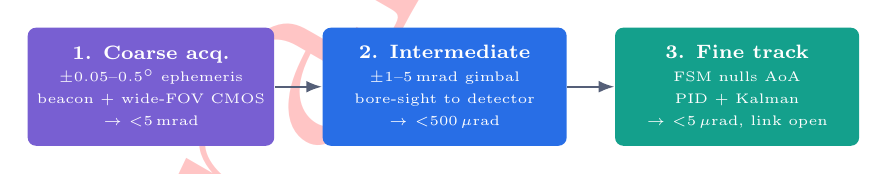
\begin{tikzpicture}[node distance=6mm]
        \node[oblk,fill=islcpurple,minimum width=3.1cm,minimum height=1.5cm](s1){\textbf{1. Coarse acq.}\\\tiny $\pm0.05$--$0.5^\circ$ ephemeris\\\tiny beacon + wide-FOV CMOS\\\tiny $\to$ $<$5\,mrad};
        \node[oblk,fill=islcblue,minimum width=3.1cm,minimum height=1.5cm,right=of s1](s2){\textbf{2. Intermediate}\\\tiny $\pm1$--5\,mrad gimbal\\\tiny bore-sight to detector\\\tiny $\to$ $<$500\,$\mu$rad};
        \node[oblk,fill=islcteal,minimum width=3.1cm,minimum height=1.5cm,right=of s2](s3){\textbf{3. Fine track}\\\tiny FSM nulls AoA\\\tiny PID + Kalman\\\tiny $\to$ $<$5\,$\mu$rad, link open};
        \draw[oarr](s1)--(s2);\draw[oarr](s2)--(s3);
    \end{tikzpicture}
    \end{center}
\end{frame}

\begin{frame}[allowframebreaks=1.2]{FSM tracking-loop design}
    \begin{itemize}
        \ai \hi{Plant} --- a lightly damped resonant mirror:
        \begin{equation*}
            P(s)=\frac{K_{act}\,\omega_n^{2}}{s^{2}+2\zeta\omega_n s+\omega_n^{2}},\quad
            \begin{aligned}
            &\omega_n = 2\pi\!\times\!500\text{--}2000\ \text{rad/s}\\
            &\zeta = 0.01\text{--}0.05,\ K_{act}=10\text{--}50\,\mu\text{rad/V}
            \end{aligned}
        \end{equation*}
        \ai \hi{Controller} $C(s)=$ PID $\times$ notches, crossover $f_c\approx300$\,Hz, phase margin $\ge45^\circ$, gain margin $\ge6$\,dB. The notch
        \begin{equation*}
            N(s)=\frac{s^{2}+2\zeta_z\omega_n s+\omega_n^{2}}{s^{2}+2\zeta_p\omega_n s+\omega_n^{2}},\quad \zeta_z\!=\!0.001,\ \zeta_p\!=\!0.3\text{--}0.5
        \end{equation*}
        places a deep null at each mechanical / reaction-wheel resonance.
    \end{itemize}
    \framebreak
    \begin{itemize}
        \ai \hi{Sensing.} 4-quadrant detector (up to 100\,kHz, $\pm$20\% spot linear range) gives the centroid error
        \begin{equation*}
            \varepsilon_x=\frac{(A+B)-(C+D)}{A+B+C+D}.
        \end{equation*}
        \ai \hi{Kalman estimator.} State $x=[\theta,\dot\theta,d_{dist}]^\mathsf{T}$ with update
        \begin{equation*}
            K_k = P_k^{-}H^\mathsf{T}\!\left(HP_k^{-}H^\mathsf{T}+R\right)^{-1},\quad R\approx(0.5\,\mu\text{rad})^2 .
        \end{equation*}
        \si Disturbance feed-forward $u_{ff}=-K_{ff}\hat d$ cancels reaction-wheel harmonics by \key{15--25\,dB} vs.\ PID alone.
    \end{itemize}
\end{frame}

%===============================================================================================
\section{Wavefront Error Budget}

\begin{frame}[allowframebreaks=1.2]{From surface to Strehl}
    \begin{itemize}
        \ai Wavefront quality maps to coupling efficiency through the \key{Mar\'echal approximation}~\cite{born1999principles}:
        \begin{equation*}
            \tcbhighmath[boxrule=1pt,arc=2pt,colback=islcteal!4,colframe=islcorange]{%
            S \approx \exp\!\left[-\left(\frac{2\pi\sigma}{\lambda}\right)^{2}\right]}
        \end{equation*}
        where $\sigma$ is the RMS wavefront error. Diffraction-limited $\equiv S>0.8$.
    \end{itemize}
    \framebreak
    \begin{block}{Representative WFE budget (RSS)}
    \centering\scriptsize
    \begin{tabular}{l r}
        \hline
        \textbf{Contributor} & \textbf{nm RMS}\\
        \hline
        Primary mirror surface figure & 11\\
        Secondary mirror figure       & 8\\
        Relay lens transmitted WFE    & 6\\
        AR/HR coating micro-roughness & 4\\
        Mirror decenter (assembly)    & 9\\
        Axial despace / focus error   & 7\\
        Thermal gradient deformation  & 12\\
        Mounting stress (flexures)    & 6\\
        Residual vibration post-FSM   & 4\\
        \hline
        \textbf{RSS total} & \textbf{23.7}\\
        \hline
    \end{tabular}
    \end{block}
    \centering Strehl $S\approx0.91 \Rightarrow$ \key{diffraction-limited} (criterion $S>0.8$).
    \framebreak
    \textbf{WFE design process --- requirement to hardware}
    \begin{enumerate}[label=\arabic*.]\footnotesize
        \item System Strehl requirement (from link budget); set target to 70\% of limit for margin.
        \item Zemax sensitivity analysis: $S_{ij}=\partial\text{WFE}_i/\partial\text{DOF}_j$ identifies dominant terms (e.g.\ secondary decenter $\to$ coma).
        \item WFE allocation: invert sensitivities, $\delta_j=\sigma_i/S_{ij}$, iterate to achievable tolerances.
        \item Manufacture \& metrology: Fizeau interferometry ($\lambda/50$), ion-beam polishing.
        \item Space qualification: TVAC, vibration, shock, TID.
        \item End-to-end link test with range-equivalent attenuation.
    \end{enumerate}
\end{frame}

%===============================================================================================
\section{CubeSat Link Budget}

\begin{frame}[allowframebreaks=1.2]{CubeSat OISL trade-space}
    \begin{equation*}
        P_{rx}=P_{tx}\,\eta_{tx}\frac{\pi D_{tx}^{2}}{4\lambda^{2}}\cdot\frac{\pi D_{rx}^{2}}{4R^{2}}\,\eta_{rx}\,L_{point}
    \end{equation*}
    \begin{columns}[T]
    \column{0.55\textwidth}
    \scriptsize
    \begin{tabular}{l r}
        \hline
        \textbf{Term (D=40\,mm, 500\,km)} & \textbf{dB}\\
        \hline
        Tx power (0.5\,W)        & $+27.0$\,dBm\\
        Tx optical eff.\ $\eta_{tx}=0.75$ & $-1.2$\\
        Tx aperture gain         & $+76.8$\\
        Free-space path loss     & $-278.2$\\
        Rx aperture (eff.\ area)  & $+67.2$\\
        Rx optical eff.\ $\eta_{rx}=0.60$ & $-2.2$\\
        Pointing loss            & $-2.0$\\
        \hline
        \textbf{Received power}  & $\mathbf{-112.6}$\,\textbf{dBm}\\
        \hline
    \end{tabular}
    \column{0.45\textwidth}
        \begin{itemize}\footnotesize
            \ai APD sensitivity @ 1\,Gbps: \hi{$-41$\,dBm}
            \ai Link margin: \hi{$+28$\,dB}
            \ai Max data rate at these params: \hi{$\sim$3\,Gbps}
        \end{itemize}
    \end{columns}
    \framebreak
    \begin{block}{The two scaling laws that govern everything}
    \footnotesize
    \key{$P_{rx}\propto D^{4}$} --- both apertures scale received power; doubling $D$ on both sides $=+12$\,dB ($\times16$). \\
    \key{$P_{rx}\propto 1/R^{2}$} --- doubling range costs 6\,dB.
    \end{block}
    \begin{itemize}\footnotesize
        \ai \hi{CubeSat limit:} 1U constrains aperture to $\sim$40--50\,mm $\Rightarrow$ Gbps+ links practical to $<$800\,km with 0.5\,W Tx.
        \ai \hi{Power tradeoff:} an EDFA at 1\,W optical draws $\sim$5--8\,W DC --- 50--80\% of a 10\,W CubeSat budget, the dominant system constraint.
    \end{itemize}
\end{frame}

%===============================================================================================
\section{Experimental Test Setup}

\begin{frame}{Experimental strategy \& test hierarchy}
    \begin{columns}[T]
    \column{0.5\textwidth}
        \begin{itemize}\footnotesize
            \ai \key{Component-level}: characterize each optical element (laser, FSM, detector, telescope) in isolation.
            \ai \key{Subsystem-level}: validate Tx chain, Rx chain and PAT loop independently.
            \ai \key{System-level}: end-to-end link with range-equivalent path loss.
            \ai \key{Environmental}: TVAC, vibration, radiation per ECSS / NASA.
        \end{itemize}
    \column{0.5\textwidth}
        \scriptsize
        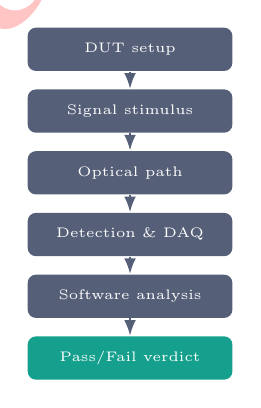
\begin{tikzpicture}[node distance=2.2mm, every node/.style={oblk,fill=islcslate,minimum width=2.6cm,minimum height=0.55cm,font=\tiny}]
            \node(a){DUT setup};
            \node[below=of a](b){Signal stimulus};
            \node[below=of b](c){Optical path};
            \node[below=of c](d){Detection \& DAQ};
            \node[below=of d](e){Software analysis};
            \node[below=of e,fill=islcteal](f){Pass/Fail verdict};
            \draw[oarr](a)--(b);\draw[oarr](b)--(c);\draw[oarr](c)--(d);\draw[oarr](d)--(e);\draw[oarr](e)--(f);
        \end{tikzpicture}
    \end{columns}
\end{frame}

\begin{frame}[allowframebreaks=1.2]{Hardware: bench, Tx \& Rx instruments}
    \textbf{Optical bench}
    \begin{itemize}\footnotesize
        \si Active-pneumatic isolation table (Newport RS2000/TMC); 6-DOF kinematic mounts (sub-$\mu$rad).
        \si 2-axis piezo mirror (PI S-330) emulates jitter; Galilean beam expander; PBS + waveplates.
        \si \key{Fizeau interferometer} ($\lambda/100$), \key{Shack--Hartmann WFS} (150 lenslets), beam profiler ($M^2$), calibrated power meter + ND set; SMF-28 delay-line emulator.
    \end{itemize}
    \framebreak
    \textbf{Tx-chain instruments}
    \begin{itemize}\footnotesize
        \si Tunable laser source (Keysight 81600B / Santec TSL-710), 1480--1640\,nm, $<$100\,kHz.
        \si Optical spectrum analyzer (Yokogawa AQ6370D), 0.02\,nm res, $>$70\,dB --- OSNR/ASE.
        \si VNA (Keysight E5063A) for MZM EO bandwidth ($>$40\,GHz); AWG (Keysight M8195A) PRBS-31 / IQ drive.
    \end{itemize}
    \framebreak
    \textbf{Rx-chain instruments}
    \begin{itemize}\footnotesize
        \si APD characterization: Keithley 2400 SMU bias, responsivity, $-3$\,dB BW, NEP (FEMTO TIA + SR830).
        \si \key{BER \& sensitivity}: BERT (Anritsu MP1800A), VOA sweep ($-25$ to $-55$\,dBm), CDR, 80\,GHz sampling scope --- read sensitivity at BER $=10^{-12}$.
    \end{itemize}
\end{frame}

\begin{frame}[allowframebreaks=1.2]{PAT test, DAQ/FPGA \& software stack}
    \textbf{PAT test hardware}
    \begin{itemize}\footnotesize
        \si Jitter emulator (PI S-330.2SL + AWG, 0--2\,mrad, 1--1000\,Hz); 4-QD (Hamamatsu G6849, $>$100\,kHz).
        \si FSM + E-727 driver ($\pm10$\,V $\to\pm5$\,mrad, $<$0.1\,$\mu$rad); coarse gimbal; CMOS InGaAs camera.
        \si \key{Real-time controller}: NI cRIO-9049 (Xilinx Kintex-7) running PID + notch + Kalman at 50--100\,kHz.
    \end{itemize}
    \framebreak
    \textbf{FPGA control loop (100\,kHz, $\sim$10\,$\mu$s budget)}
    \begin{enumerate}[label=\arabic*.]\scriptsize
        \item ADC read 4-QD $\to$ centroid error (10\,$\mu$s)
        \item Bandpass error filter, 100--800\,Hz (1\,$\mu$s)
        \item Velocity-form PID (2\,$\mu$s)
        \item IIR notch sections at $\omega_n$, $f_{RW}$, $2f_{RW}$, $3f_{RW}$ (2\,$\mu$s)
        \item Kalman predict + disturbance feed-forward (3\,$\mu$s)
        \item DAC write to FSM, saturated at $\pm9.5$\,V (2\,$\mu$s)
    \end{enumerate}
    \framebreak
    \textbf{Software layers}
    \begin{itemize}\footnotesize
        \si L5 Analysis: Python/MATLAB --- NumPy, SciPy, matplotlib, pandas.
        \si L4 Orchestration: LabVIEW TestStand / pytest, SCPI drivers, CI.
        \si L3 Real-time: LabVIEW RT / Simulink RT --- PAT state machine, Kalman.
        \si L2 FPGA: VHDL/Vivado --- PID + notch, 100\,kHz.
        \si L1 Drivers: NI-VISA / NI-DAQmx, SCPI over GPIB/USB/LAN.
    \end{itemize}
\end{frame}

\begin{frame}{Integrated hardware + software test chain}
    \begin{center}
    \scriptsize
    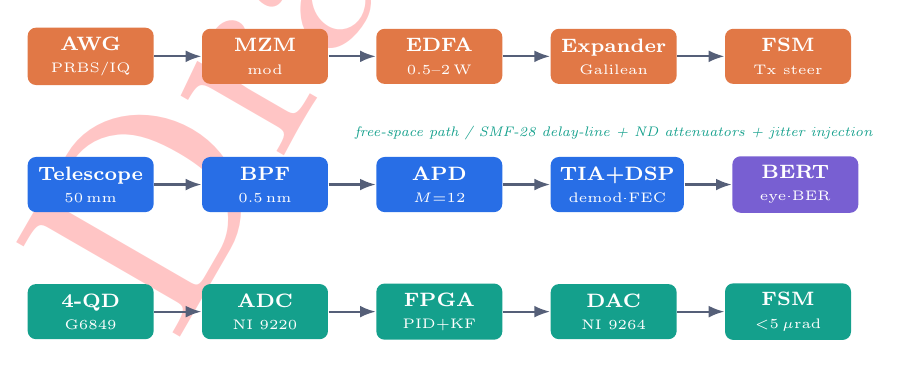
\begin{tikzpicture}[node distance=2.5mm and 6mm]
        % Tx row
        \node[oblk,fill=islcorange,minimum width=1.6cm,minimum height=0.7cm](awg){\textbf{AWG}\\\tiny PRBS/IQ};
        \node[oblk,fill=islcorange,minimum width=1.6cm,minimum height=0.7cm,right=of awg](mzm){\textbf{MZM}\\\tiny mod};
        \node[oblk,fill=islcorange,minimum width=1.6cm,minimum height=0.7cm,right=of mzm](edfa){\textbf{EDFA}\\\tiny 0.5--2\,W};
        \node[oblk,fill=islcorange,minimum width=1.6cm,minimum height=0.7cm,right=of edfa](be){\textbf{Expander}\\\tiny Galilean};
        \node[oblk,fill=islcorange,minimum width=1.6cm,minimum height=0.7cm,right=of be](fsm1){\textbf{FSM}\\\tiny Tx steer};
        \draw[oarr](awg)--(mzm);\draw[oarr](mzm)--(edfa);\draw[oarr](edfa)--(be);\draw[oarr](be)--(fsm1);
        % channel
        \node[below=4mm of be, text=islcteal, font=\tiny\itshape](ch){free-space path / SMF-28 delay-line + ND attenuators + jitter injection};
        % Rx row
        \node[oblk,fill=islcblue,minimum width=1.6cm,minimum height=0.7cm,below=9mm of awg](tele){\textbf{Telescope}\\\tiny 50\,mm};
        \node[oblk,fill=islcblue,minimum width=1.6cm,minimum height=0.7cm,right=of tele](bpf){\textbf{BPF}\\\tiny 0.5\,nm};
        \node[oblk,fill=islcblue,minimum width=1.6cm,minimum height=0.7cm,right=of bpf](apd){\textbf{APD}\\\tiny $M{=}12$};
        \node[oblk,fill=islcblue,minimum width=1.6cm,minimum height=0.7cm,right=of apd](tia){\textbf{TIA+DSP}\\\tiny demod·FEC};
        \node[oblk,fill=islcpurple,minimum width=1.6cm,minimum height=0.7cm,right=of tia](bert){\textbf{BERT}\\\tiny eye·BER};
        \draw[oarr](tele)--(bpf);\draw[oarr](bpf)--(apd);\draw[oarr](apd)--(tia);\draw[oarr](tia)--(bert);
        % PAT row
        \node[oblk,fill=islcteal,minimum width=1.6cm,minimum height=0.7cm,below=9mm of tele](qd){\textbf{4-QD}\\\tiny G6849};
        \node[oblk,fill=islcteal,minimum width=1.6cm,minimum height=0.7cm,right=of qd](adc){\textbf{ADC}\\\tiny NI 9220};
        \node[oblk,fill=islcteal,minimum width=1.6cm,minimum height=0.7cm,right=of adc](fpga){\textbf{FPGA}\\\tiny PID+KF};
        \node[oblk,fill=islcteal,minimum width=1.6cm,minimum height=0.7cm,right=of fpga](dac){\textbf{DAC}\\\tiny NI 9264};
        \node[oblk,fill=islcteal,minimum width=1.6cm,minimum height=0.7cm,right=of dac](fsm2){\textbf{FSM}\\\tiny $<$5\,$\mu$rad};
        \draw[oarr](qd)--(adc);\draw[oarr](adc)--(fpga);\draw[oarr](fpga)--(dac);\draw[oarr](dac)--(fsm2);
    \end{tikzpicture}
    \end{center}
    \footnotesize Top: transmit side. Middle: emulated channel. Bottom: closed PAT tracking loop.
\end{frame}

\begin{frame}{Key measurement sequences \& acceptance criteria}
    \footnotesize
    \begin{columns}[T]
    \column{0.33\textwidth}
        \textbf{WFE \& Strehl}
        \begin{itemize}\scriptsize
            \si SH-WFS, 100 frames, Zernike Z4--Z37
            \si RSS WFE; Strehl via Mar\'echal
        \end{itemize}
        \textcolor{islcteal}{$\checkmark$ RSS WFE $<$30\,nm, $S>0.80$}
    \column{0.33\textwidth}
        \textbf{FSM loop closure}
        \begin{itemize}\scriptsize
            \si Swept-sine $\to$ $H(f)$, fit $\omega_n,\zeta$
            \si PID+notch, inject 60/120/180\,Hz
        \end{itemize}
        \textcolor{islcteal}{$\checkmark$ RMS $<$5\,$\mu$rad, BW $>$500\,Hz}
    \column{0.33\textwidth}
        \textbf{BER waterfall}
        \begin{itemize}\scriptsize
            \si Sweep VOA, fit $0.5\,\mathrm{erfc}(Q/\sqrt2)$
            \si Margin $\ge3$\,dB
        \end{itemize}
        \textcolor{islcteal}{$\checkmark$ $\le-35$\,dBm @ 10G, $10^{-12}$}
    \end{columns}
    \vspace{2mm}
    \begin{block}{Environmental qualification}
    \scriptsize TVAC ($<10^{-6}$\,mbar, $-40$ to $+70^\circ$C, in-situ WFS) --- WFE RSS $<$35\,nm, $S>0.78$. \quad
    Vibration (GEVS-7000A, 14.1\,$g_{rms}$) + 3000\,g shock. \quad Co-60 TID (10--50\,krad Si) on EDFA fiber \& APD.
    \end{block}
\end{frame}

%===============================================================================================
\section{Flown Hardware \& Conclusion}

\begin{frame}{Reference CubeSat-class terminals}
    \begin{columns}[T]
    \column{0.5\textwidth}
        \begin{block}{CLICK-B/C~\cite{cahoy2020click}}
        \footnotesize MIT / UF / NASA
        \begin{itemize}\scriptsize
            \si Two 3U CubeSats; sub-2U terminals
            \si 20\,Mbps full-duplex, 25--580\,km
            \si 1537/1563\,nm, $\sim$200\,mW, direct detection
            \si MEMS fast-steering mirror \& ranging
        \end{itemize}
        \end{block}
    \column{0.5\textwidth}
        \begin{block}{TBIRD~\cite{robinson2018tbird,schieler2023tbird}}
        \footnotesize MIT Lincoln Laboratory
        \begin{itemize}\scriptsize
            \si 3U payload on a 6U bus
            \si 100 / 200\,Gbps downlink to ground
            \si Coherent fiber-coupled COTS transceivers
            \si ARQ error-free delivery --- up to 4.8\,TB/pass
        \end{itemize}
        \end{block}
    \end{columns}
    \vspace{2mm}
    \centering\footnotesize Interoperability is converging on the SDA \key{Optical Communications Terminal (OCT)} standard~\cite{sda2022oct}.
\end{frame}

\begin{frame}{Key takeaways}
    \begin{itemize}
        \ai OISL is the \key{laser backbone} of modern constellations --- vast gain and bandwidth from a tiny aperture~\cite{kaushal2017optical,toyoshima2021trends}.
        \ai The narrow beam makes \hi{pointing, not photons,} the dominant engineering risk.
        \ai The link budget governs everything: \key{$P_{rx}\propto D^{4}$} --- aperture is the highest-leverage variable.
        \ai Point-ahead, Tx/Rx isolation and FSM jitter rejection are the defining sub-problems; the \key{FSM tracking loop} (PID + notch, $>$500\,Hz, Kalman) is the critical control subsystem.
        \ai CubeSat-scale OISL ($<$50\,mm, $<$1\,W, 1U) enables \key{Gbps+ at $<$800\,km} --- feasible today. Frontiers: MEMS FSM, photonic-IC transceivers, coherent QPSK.
    \end{itemize}
\end{frame}

%-----------------------------------------------------------------------------------------------
\begin{frame}{}
    \centering
    \vfill
    {\fontsize{22}{26}\selectfont \textcolor{islcteal}{\textbf{Thank you}}}\\[4mm]
    {\large Questions \& discussion}
    \vfill
\end{frame}
%-----------------------------------------------------------------------------------------------
\begin{frame}[allowframebreaks=0.9]{References}
    \bibliographystyle{model1-num-names}
    \bibliography{cas-refs}
    \framebreak
\end{frame}
%-----------------------------------------------------------------------------------------------
\end{document}



% These "\usepackage{}" commands import packages into the LaTeX document.
\usepackage[english]{babel}
\usepackage[light,math]{anttor}
\usepackage{graphicx,graphbox}
\usepackage{parskip}
\usepackage{amsmath}
\usepackage{caption}
\usepackage{subcaption}
\usepackage{background}
\usepackage{xcolor}

\usepackage[skins, theorems]{tcolorbox}
\usepackage{pifont}
\usepackage{amssymb,enumitem}
\usepackage{indentfirst}
\usepackage{tabularray}
\usepackage{hyperref}
\usepackage{cleveref}
\usepackage{array}
\usepackage{multirow}
\setbeamertemplate{caption}[numbered]
\usepackage[square,numbers,sort&compress]{natbib}
\renewcommand{\bibsection}{\subsubsection*{\bibname}}
\setbeamertemplate{frametitle continuation}[from second][(contd.)]
\usepackage{setspace}
\onehalfspacing

% Extra TikZ libraries for the block diagrams (tikz + positioning come from the class)
\usetikzlibrary{arrows.meta,positioning,shapes.geometric,fit,backgrounds,calc}

\usetheme{Madrid}
\usecolortheme{default}
\hypersetup{
    colorlinks=true,
    linkcolor=cyan,
    urlcolor=cyan,
    citecolor=cyan,
}

%------------------------------------------------------------
% ISLC colour palette (complements the kaist-* colours from the class)
\definecolor{islcteal}{RGB}{20,160,140}
\definecolor{islcblue}{RGB}{40,110,230}
\definecolor{islcorange}{RGB}{225,120,70}
\definecolor{islcslate}{RGB}{85,95,120}
\definecolor{islcpurple}{RGB}{120,95,210}

% Shorthand bullets and highlight macros to keep the body readable
\newcommand{\ai}{\item[\textcolor{islcteal}{\ding{228}}]}      % primary bullet
\newcommand{\si}{\item[\textcolor{islcorange}{\ding{167}}]}    % sub bullet
\newcommand{\hi}[1]{\textcolor{islcorange}{\textbf{#1}}}       % inline highlight
\newcommand{\key}[1]{\textcolor{islcblue}{\textbf{#1}}}        % inline key term

% Generic TikZ block styles for the architecture / chain diagrams
\tikzset{
  oblk/.style={rectangle, rounded corners=3pt, draw=none, text=white,
               align=center, font=\scriptsize, minimum width=2.6cm, minimum height=1.15cm},
  oarr/.style={-{Latex[length=2mm]}, thick, islcslate},
}

%------------------------------------------------------------
% Title-page information
\title[ISLC for CubeSats] %optional
{Inter-Satellite Laser Communication for CubeSat Platforms}

\subtitle{Optical terminal architecture, design \& experimental setup}

\author[Dinaol Gadisa] % (optional)
{Dinaol Gadisa\inst{1} \and Hyochoong Bang\inst{1}}

\institute[ASCL] % (optional)
{
  \inst{1}%
  Aerospace System and Control Lab, Department of Aerospace Engineering, KAIST\\
}

\date[ASCL-P2026] % (optional)
{ISLC research report, June 2026}

%End of title-page configuration block
%------------------------------------------------------------

% Put a table of contents at the start of every section
\AtBeginSection[]
{
  \begin{frame}
    \frametitle{Table of Contents}
    \tableofcontents[currentsection]
  \end{frame}
}

\renewcommand{\titlelogo}{logo/ascl logo.svg}
\renewcommand{\slidelogo}{logo/ascl logo.svg}
% If \includesvg is unavailable, drop the extension and use a raster logo instead:
% \renewcommand{\titlelogo}{logo/ascl logo}
% \renewcommand{\slidelogo}{logo/ascl logo}

\backgroundsetup{
  scale=0.6,
  angle=0,
  opacity=0.02,
  contents={
    
\includegraphics[width=\textwidth,height=\textwidth]{figs/download.png}}
}

\renewcommand{\slidefoot}{Dinaol Gadisa}
%-----------------------------------------------------------------------------------------------
\begin{document}

\frame{\titlepage}

%===============================================================================================
\section{Introduction \& Motivation}

\begin{frame}[t,allowframebreaks=1.2]{Why optical inter-satellite links?}
    \begin{itemize}
        \ai Inter-satellite laser communication (\hi{ISLC}, also \hi{OISL}) links satellites \key{directly} to one another with laser beams instead of routing every bit down to the ground and back up~\cite{kaushal2017optical,sodnik2010optical}.
        \ai The carrier is a near-infrared laser --- typically \key{1550\,nm} ($\sim$193\,THz) --- inherited from the fiber-telecom ecosystem.
        \ai Chained across a constellation, the links form a \key{low-latency optical mesh} that moves data in orbit --- the in-space backbone of Starlink, Kuiper and the SDA transport layer~\cite{chaudhry2021free,sda2022oct}.
    \end{itemize}
    \framebreak
    \begin{block}{Optical vs.\ RF --- why lasers win in space~\cite{kaushal2017optical}}
    \centering\footnotesize
    \begin{tabular}{l l l}
        \hline
        \textbf{Parameter} & \textbf{Ka-band RF} & \textbf{OISL @ 1550\,nm}\\
        \hline
        Data rate      & 100--600\,Mbps   & 1--100\,Gbps\\
        Carrier        & 26--40\,GHz      & $\sim$193\,THz\\
        Beam divergence& $\sim0.5$--$2^\circ$ & $\sim$10--100\,$\mu$rad\\
        Aperture       & 200--600\,mm     & 30--100\,mm\\
        Licensing      & \textcolor{red}{Required} & \textcolor{islcteal}{None (LPI/LPD)}\\
        \hline
    \end{tabular}
    \end{block}
    \begin{itemize}
        \ai \hi{The catch:} a tens-of-$\mu$rad beam must be pointed to a few $\mu$rad across thousands of km --- \key{pointing, not photons, is the hard problem}.
    \end{itemize}
\end{frame}

\begin{frame}{Advantages of OISL}
    \begin{columns}[T]
    \column{0.5\textwidth}
        \begin{itemize}
            \ai \hi{10--100$\times$} higher data rate than Ka-band RF
            \ai \hi{$\sim$10\,$\mu$rad} beam divergence (vs.\ $\sim1^\circ$ for RF)
            \ai \hi{No ITU} frequency licensing required
            \ai \hi{$<$50\%} mass \& aperture vs.\ equivalent RF
        \end{itemize}
    \column{0.5\textwidth}
        \begin{block}{CubeSat relevance~\cite{toyoshima2021trends,cahoy2020click}}
        A 50\,mm-aperture OISL achieves \key{Gbps at 500\,km} in a $\sim$0.5U volume --- impossible with RF in the same form factor.
        \end{block}
    \end{columns}
\end{frame}

%===============================================================================================
\section{Link Fundamentals}

\begin{frame}[allowframebreaks=1.2]{The link in one equation}
    \begin{itemize}
        \ai The received power follows the free-space optical link equation~\cite{hemmati2009near,caplan2007laser}:
    \end{itemize}
    \begin{equation*}
        \tcbhighmath[boxrule=1pt,arc=2pt,colback=islcteal!4,colframe=islcblue,drop fuzzy shadow=islcslate]{%
        P_{rx} = P_{tx}\, G_{tx}\, \left(\frac{\lambda}{4\pi R}\right)^{2} G_{rx}\, L_{point}\, L_{impl}}
    \end{equation*}
    \begin{itemize}
        \si \hi{Aperture gain} $G = (\pi D/\lambda)^2 \approx +100$\,dB for a diffraction-limited 5\,cm telescope.
        \si \hi{Free-space loss} $(\lambda/4\pi R)^2 \approx -262$\,dB over 1500\,km at 1550\,nm.
        \si \hi{Pointing loss} $\propto e^{-2(\theta/\theta_0)^2}$ --- $\tfrac13$ of a beamwidth off $\approx$ 1\,dB lost.
    \end{itemize}
    \framebreak
    \begin{itemize}
        \ai Two competing quantities set everything: \key{antenna gain} and \key{beam divergence}
        \begin{equation*}
            G = \left(\frac{\pi D}{\lambda}\right)^{2}, \qquad \theta \approx \frac{\lambda}{D}\approx\frac{\lambda}{\pi w_0}.
        \end{equation*}
        \ai Enormous gains fight an enormous path loss; \key{sensitivity} is then set by \hi{photons/bit}:
        \begin{equation*}
            P_{req} = \left(\frac{\text{photons}}{\text{bit}}\right)\frac{hc}{\lambda}\,R_b .
        \end{equation*}
        \si OOK $\approx$ tens, DPSK $\approx 38$, coherent $\approx 9$ photons/bit at BER $10^{-9}$~\cite{caplan2007laser}.
    \end{itemize}
\end{frame}

%===============================================================================================
\section{Optical Terminal Architecture}

\begin{frame}{Terminal architecture at a glance}
    \begin{center}
    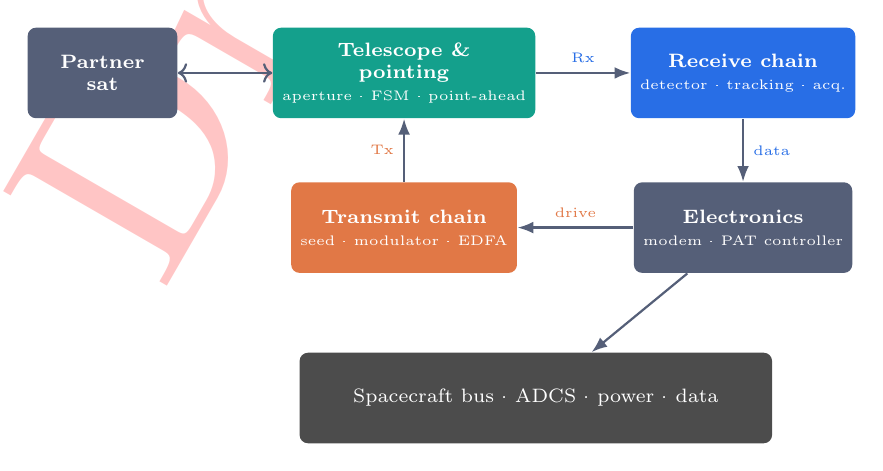
\begin{tikzpicture}[node distance=8mm and 12mm]
        \node[oblk, fill=islcslate, minimum width=1.9cm](sat){\textbf{Partner}\\\textbf{sat}};
        \node[oblk, fill=islcteal, right=of sat](tel){\textbf{Telescope \&}\\\textbf{pointing}\\\tiny aperture · FSM · point-ahead};
        \node[oblk, fill=islcblue, right=of tel](rx){\textbf{Receive chain}\\\tiny detector · tracking · acq.};
        \node[oblk, fill=islcorange, below=of tel](tx){\textbf{Transmit chain}\\\tiny seed · modulator · EDFA};
        \node[oblk, fill=islcslate, below=of rx](el){\textbf{Electronics}\\\tiny modem · PAT controller};
        \node[oblk, fill=black!70, minimum width=6cm, below=10mm of el.south -| tel.east](bus){\scriptsize Spacecraft bus · ADCS · power · data};

        \draw[oarr,<->](sat)--(tel);
        \draw[oarr](tel)-- node[above,font=\tiny,text=islcblue]{Rx} (rx);
        \draw[oarr](rx)-- node[right,font=\tiny,text=islcblue]{data} (el);
        \draw[oarr](el)-- node[above,font=\tiny,text=islcorange]{drive} (tx);
        \draw[oarr](tx.north)-- node[left,font=\tiny,text=islcorange]{Tx} (tel.south);
        \draw[oarr](el)--(bus);
    \end{tikzpicture}
    \end{center}
    \footnotesize Four blocks around \key{one shared aperture} that transmits watts, receives nanowatts and steers to microradians~\cite{sodnik2010optical}.
\end{frame}

\begin{frame}[allowframebreaks=1.2]{Aperture, transmit \& receive chains}
    \begin{itemize}
        \ai \hi{Aperture \& telescope.} A single aperture is shared by Tx and Rx to save mass; the hard part is \key{Tx/Rx isolation} --- $\sim$1\,W out vs.\ $\sim$10\,nW in is an 80--100\,dB dynamic range, won by wavelength offset (e.g.\ 1537/1563\,nm), polarization, or time-division.
    \end{itemize}
    \framebreak
    \textbf{Transmit chain} --- a fiber-laser (MOPA) stack:
    \begin{center}
    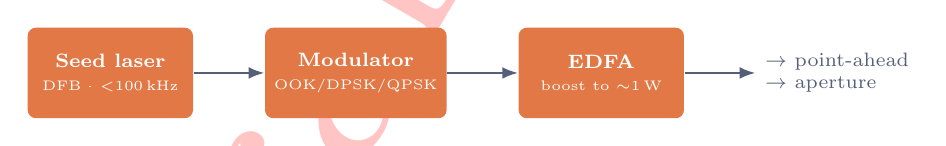
\begin{tikzpicture}[node distance=5mm and 9mm]
        \node[oblk, fill=islcorange, minimum width=2.1cm](seed){\textbf{Seed laser}\\\tiny DFB · $<$100\,kHz};
        \node[oblk, fill=islcorange, minimum width=2.1cm, right=of seed](mod){\textbf{Modulator}\\\tiny OOK/DPSK/QPSK};
        \node[oblk, fill=islcorange, minimum width=2.1cm, right=of mod](edfa){\textbf{EDFA}\\\tiny boost to $\sim$1\,W};
        \node[right=of edfa, font=\scriptsize, align=left, text=islcslate](out){$\rightarrow$ point-ahead\\$\rightarrow$ aperture};
        \draw[oarr](seed)--(mod);\draw[oarr](mod)--(edfa);\draw[oarr](edfa)--(out);
    \end{tikzpicture}
    \end{center}
    \framebreak
    \textbf{Receive chain} --- the incoming beam is tapped three ways:
    \begin{center}
    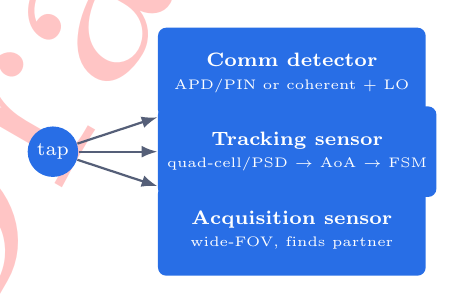
\begin{tikzpicture}[node distance=4mm and 10mm]
        \node[circle,fill=islcblue,text=white,font=\scriptsize,inner sep=2pt](tap){tap};
        \node[oblk, fill=islcblue, right=of tap, yshift=10mm, minimum width=3.4cm](comm){\textbf{Comm detector}\\\tiny APD/PIN or coherent + LO};
        \node[oblk, fill=islcblue, right=of tap, minimum width=3.4cm](trk){\textbf{Tracking sensor}\\\tiny quad-cell/PSD $\to$ AoA $\to$ FSM};
        \node[oblk, fill=islcblue, right=of tap, yshift=-10mm, minimum width=3.4cm](acq){\textbf{Acquisition sensor}\\\tiny wide-FOV, finds partner};
        \draw[oarr](tap)--(comm);\draw[oarr](tap)--(trk);\draw[oarr](tap)--(acq);
    \end{tikzpicture}
    \end{center}
    \framebreak
    \begin{itemize}
        \ai \hi{Electronics \& control.} The \key{modem} runs FEC (LDPC), framing and an ARQ retransmit layer for error-free delivery through fades; the \key{PAT controller} runs the nested acquisition/tracking loops, computes point-ahead and closes the FSM loop.
        \ai It also handles \key{Doppler}: at 1550\,nm a 15\,km/s closing rate shifts the carrier by $\sim$10\,GHz, tracked by an AFC loop on coherent systems.
    \end{itemize}
\end{frame}

%===============================================================================================
\section{Optical Components}

\begin{frame}[allowframebreaks=1.2]{Laser source \& modulation}
    \begin{columns}[T]
    \column{0.52\textwidth}
        \textbf{MOPA laser source}
        \begin{itemize}\footnotesize
            \si $\lambda = 1550$\,nm (eye-safe, EDFA band)
            \si DFB seed, linewidth $<100$\,kHz
            \si 10--40\,mW seed $\to$ 0.5--5\,W via EDFA
            \si Linear polarization (MZM requirement)
            \si RIN $< -150$\,dB/Hz; rad-hard Er-fiber
        \end{itemize}
    \column{0.48\textwidth}
        \textbf{Modulation formats}~\cite{caplan2007laser}
        \begin{itemize}\footnotesize
            \si \key{OOK}: simple, $\sim-28$\,dBm @ 10G
            \si \key{DPSK}: +3\,dB, $\sim-31$\,dBm @ 10G
            \si \key{QPSK}: coherent, $\sim-35$\,dBm @ 10G
        \end{itemize}
    \end{columns}
    \vspace{2mm}
    \begin{block}{Doppler challenge @ 1550\,nm}
    Two LEO satellites at 7.5\,km/s $\Rightarrow$ $\Delta f = f\,v/c \approx 5$\,GHz Doppler shift $\Rightarrow$ requires optical pre-compensation / AFC in the PAT loop.
    \end{block}
\end{frame}

\begin{frame}[allowframebreaks=1.2]{Beam expander, FSM \& detector}
    \begin{columns}[T]
    \column{0.5\textwidth}
        \textbf{Beam expander (Tx telescope)}
        \begin{itemize}\footnotesize
            \si Galilean afocal (no focus $\to$ no air breakdown)
            \si $D = 30$--80\,mm; CubeSat $\sim$50\,mm
            \si $\theta \approx \lambda/(\pi w_0)\approx40\,\mu$rad @ 50\,mm
            \si $\sim$20\,m footprint @ 500\,km (vs.\ 4\,km Ka)
            \si Strehl $>0.8 \Rightarrow$ WFE $<\lambda/14=111$\,nm RMS
        \end{itemize}
    \column{0.5\textwidth}
        \textbf{Fine steering mirror (FSM)}
        \begin{itemize}\footnotesize
            \si 15--30\,mm clear aperture, PZT or VCA
            \si Range $\pm1$--5\,mrad, resolution $<1\,\mu$rad
            \si Bandwidth $>500$\,Hz to reject RW harmonics
            \si Shared by Tx pointing \& PAT correction
        \end{itemize}
    \end{columns}
    \framebreak
    \begin{block}{Photodetectors}
    \footnotesize
    \key{InGaAs APD} (workhorse, LEO--LEO): gain $M=5$--20, $-30$ to $-35$\,dBm @ 10G, room temperature, 900--1650\,nm. \quad
    \key{SNSPD} (deep-space, photon-starved): single-photon, $>$90\% efficiency, $<$50\,ps jitter --- flown on NASA LLCD~\cite{boroson2014llcd}.
    \end{block}
    \begin{center}\scriptsize
    
\begin{tikzpicture}[node distance=3mm and 6mm]
        \node[oblk,fill=islcteal,minimum width=1.7cm](t){\textbf{Cassegrain}\\\tiny 50--100\,mm};
        \node[oblk,fill=islcteal,minimum width=1.7cm,right=of t](f){\textbf{BPF}\\\tiny 0.3--1\,nm};
        \node[oblk,fill=islcteal,minimum width=1.7cm,right=of f](fo){\textbf{Focus}\\\tiny f/4--f/8};
        \node[oblk,fill=islcteal,minimum width=1.7cm,right=of fo](apd){\textbf{APD}\\\tiny $M{=}10$--15};
        \node[oblk,fill=islcteal,minimum width=1.7cm,right=of apd](dsp){\textbf{TIA+DSP}\\\tiny demod·FEC};
        \draw[oarr](t)--(f);\draw[oarr](f)--(fo);\draw[oarr](fo)--(apd);\draw[oarr](apd)--(dsp);
    \end{tikzpicture}
    \end{center}
    \centering\footnotesize Complete receive chain. \quad Key coupling: $\theta\propto\lambda/D$ --- larger aperture $=$ narrower beam $=$ higher gain $=$ tighter pointing requirement.
\end{frame}

%===============================================================================================
\section{Pointing, Acquisition \& Tracking}

\begin{frame}[allowframebreaks=1.2]{Point-ahead \& acquisition}
    \begin{itemize}
        \ai Light takes time to cross the link and both satellites move --- you transmit toward where the partner \key{WILL be} while its beam arrives from where it \key{WAS}~\cite{kaushal2017optical}.
        \ai The lead angle is
        \begin{equation*}
            \alpha_{PA}\approx \frac{2v_\perp}{c}.
        \end{equation*}
        \si Cross-plane LEO: $v_\perp$ up to $\sim$15\,km/s gives $\sim$100\,$\mu$rad --- comparable to the whole beamwidth, so a dedicated actuator is required.
        \si Same-plane crosslinks move together: point-ahead nearly vanishes.
    \end{itemize}
    \framebreak
    \textbf{From blind to locked --- 3-stage PAT}
    \begin{center}
    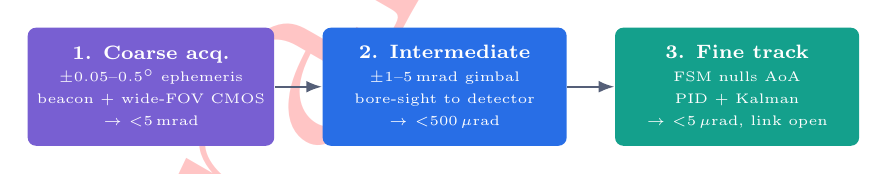
\begin{tikzpicture}[node distance=6mm]
        \node[oblk,fill=islcpurple,minimum width=3.1cm,minimum height=1.5cm](s1){\textbf{1. Coarse acq.}\\\tiny $\pm0.05$--$0.5^\circ$ ephemeris\\\tiny beacon + wide-FOV CMOS\\\tiny $\to$ $<$5\,mrad};
        \node[oblk,fill=islcblue,minimum width=3.1cm,minimum height=1.5cm,right=of s1](s2){\textbf{2. Intermediate}\\\tiny $\pm1$--5\,mrad gimbal\\\tiny bore-sight to detector\\\tiny $\to$ $<$500\,$\mu$rad};
        \node[oblk,fill=islcteal,minimum width=3.1cm,minimum height=1.5cm,right=of s2](s3){\textbf{3. Fine track}\\\tiny FSM nulls AoA\\\tiny PID + Kalman\\\tiny $\to$ $<$5\,$\mu$rad, link open};
        \draw[oarr](s1)--(s2);\draw[oarr](s2)--(s3);
    \end{tikzpicture}
    \end{center}
\end{frame}

\begin{frame}[allowframebreaks=1.2]{FSM tracking-loop design}
    \begin{itemize}
        \ai \hi{Plant} --- a lightly damped resonant mirror:
        \begin{equation*}
            P(s)=\frac{K_{act}\,\omega_n^{2}}{s^{2}+2\zeta\omega_n s+\omega_n^{2}},\quad
            \begin{aligned}
            &\omega_n = 2\pi\!\times\!500\text{--}2000\ \text{rad/s}\\
            &\zeta = 0.01\text{--}0.05,\ K_{act}=10\text{--}50\,\mu\text{rad/V}
            \end{aligned}
        \end{equation*}
        \ai \hi{Controller} $C(s)=$ PID $\times$ notches, crossover $f_c\approx300$\,Hz, phase margin $\ge45^\circ$, gain margin $\ge6$\,dB. The notch
        \begin{equation*}
            N(s)=\frac{s^{2}+2\zeta_z\omega_n s+\omega_n^{2}}{s^{2}+2\zeta_p\omega_n s+\omega_n^{2}},\quad \zeta_z\!=\!0.001,\ \zeta_p\!=\!0.3\text{--}0.5
        \end{equation*}
        places a deep null at each mechanical / reaction-wheel resonance.
    \end{itemize}
    \framebreak
    \begin{itemize}
        \ai \hi{Sensing.} 4-quadrant detector (up to 100\,kHz, $\pm$20\% spot linear range) gives the centroid error
        \begin{equation*}
            \varepsilon_x=\frac{(A+B)-(C+D)}{A+B+C+D}.
        \end{equation*}
        \ai \hi{Kalman estimator.} State $x=[\theta,\dot\theta,d_{dist}]^\mathsf{T}$ with update
        \begin{equation*}
            K_k = P_k^{-}H^\mathsf{T}\!\left(HP_k^{-}H^\mathsf{T}+R\right)^{-1},\quad R\approx(0.5\,\mu\text{rad})^2 .
        \end{equation*}
        \si Disturbance feed-forward $u_{ff}=-K_{ff}\hat d$ cancels reaction-wheel harmonics by \key{15--25\,dB} vs.\ PID alone.
    \end{itemize}
\end{frame}

%===============================================================================================
\section{Wavefront Error Budget}

\begin{frame}[allowframebreaks=1.2]{From surface to Strehl}
    \begin{itemize}
        \ai Wavefront quality maps to coupling efficiency through the \key{Mar\'echal approximation}~\cite{born1999principles}:
        \begin{equation*}
            \tcbhighmath[boxrule=1pt,arc=2pt,colback=islcteal!4,colframe=islcorange]{%
            S \approx \exp\!\left[-\left(\frac{2\pi\sigma}{\lambda}\right)^{2}\right]}
        \end{equation*}
        where $\sigma$ is the RMS wavefront error. Diffraction-limited $\equiv S>0.8$.
    \end{itemize}
    \framebreak
    \begin{block}{Representative WFE budget (RSS)}
    \centering\scriptsize
    \begin{tabular}{l r}
        \hline
        \textbf{Contributor} & \textbf{nm RMS}\\
        \hline
        Primary mirror surface figure & 11\\
        Secondary mirror figure       & 8\\
        Relay lens transmitted WFE    & 6\\
        AR/HR coating micro-roughness & 4\\
        Mirror decenter (assembly)    & 9\\
        Axial despace / focus error   & 7\\
        Thermal gradient deformation  & 12\\
        Mounting stress (flexures)    & 6\\
        Residual vibration post-FSM   & 4\\
        \hline
        \textbf{RSS total} & \textbf{23.7}\\
        \hline
    \end{tabular}
    \end{block}
    \centering Strehl $S\approx0.91 \Rightarrow$ \key{diffraction-limited} (criterion $S>0.8$).
    \framebreak
    \textbf{WFE design process --- requirement to hardware}
    \begin{enumerate}[label=\arabic*.]\footnotesize
        \item System Strehl requirement (from link budget); set target to 70\% of limit for margin.
        \item Zemax sensitivity analysis: $S_{ij}=\partial\text{WFE}_i/\partial\text{DOF}_j$ identifies dominant terms (e.g.\ secondary decenter $\to$ coma).
        \item WFE allocation: invert sensitivities, $\delta_j=\sigma_i/S_{ij}$, iterate to achievable tolerances.
        \item Manufacture \& metrology: Fizeau interferometry ($\lambda/50$), ion-beam polishing.
        \item Space qualification: TVAC, vibration, shock, TID.
        \item End-to-end link test with range-equivalent attenuation.
    \end{enumerate}
\end{frame}

%===============================================================================================
\section{CubeSat Link Budget}

\begin{frame}[allowframebreaks=1.2]{CubeSat OISL trade-space}
    \begin{equation*}
        P_{rx}=P_{tx}\,\eta_{tx}\frac{\pi D_{tx}^{2}}{4\lambda^{2}}\cdot\frac{\pi D_{rx}^{2}}{4R^{2}}\,\eta_{rx}\,L_{point}
    \end{equation*}
    \begin{columns}[T]
    \column{0.55\textwidth}
    \scriptsize
    \begin{tabular}{l r}
        \hline
        \textbf{Term (D=40\,mm, 500\,km)} & \textbf{dB}\\
        \hline
        Tx power (0.5\,W)        & $+27.0$\,dBm\\
        Tx optical eff.\ $\eta_{tx}=0.75$ & $-1.2$\\
        Tx aperture gain         & $+76.8$\\
        Free-space path loss     & $-278.2$\\
        Rx aperture (eff.\ area)  & $+67.2$\\
        Rx optical eff.\ $\eta_{rx}=0.60$ & $-2.2$\\
        Pointing loss            & $-2.0$\\
        \hline
        \textbf{Received power}  & $\mathbf{-112.6}$\,\textbf{dBm}\\
        \hline
    \end{tabular}
    \column{0.45\textwidth}
        \begin{itemize}\footnotesize
            \ai APD sensitivity @ 1\,Gbps: \hi{$-41$\,dBm}
            \ai Link margin: \hi{$+28$\,dB}
            \ai Max data rate at these params: \hi{$\sim$3\,Gbps}
        \end{itemize}
    \end{columns}
    \framebreak
    \begin{block}{The two scaling laws that govern everything}
    \footnotesize
    \key{$P_{rx}\propto D^{4}$} --- both apertures scale received power; doubling $D$ on both sides $=+12$\,dB ($\times16$). \\
    \key{$P_{rx}\propto 1/R^{2}$} --- doubling range costs 6\,dB.
    \end{block}
    \begin{itemize}\footnotesize
        \ai \hi{CubeSat limit:} 1U constrains aperture to $\sim$40--50\,mm $\Rightarrow$ Gbps+ links practical to $<$800\,km with 0.5\,W Tx.
        \ai \hi{Power tradeoff:} an EDFA at 1\,W optical draws $\sim$5--8\,W DC --- 50--80\% of a 10\,W CubeSat budget, the dominant system constraint.
    \end{itemize}
\end{frame}

%===============================================================================================
\section{Experimental Test Setup}

\begin{frame}{Experimental strategy \& test hierarchy}
    \begin{columns}[T]
    \column{0.5\textwidth}
        \begin{itemize}\footnotesize
            \ai \key{Component-level}: characterize each optical element (laser, FSM, detector, telescope) in isolation.
            \ai \key{Subsystem-level}: validate Tx chain, Rx chain and PAT loop independently.
            \ai \key{System-level}: end-to-end link with range-equivalent path loss.
            \ai \key{Environmental}: TVAC, vibration, radiation per ECSS / NASA.
        \end{itemize}
    \column{0.5\textwidth}
        \scriptsize
        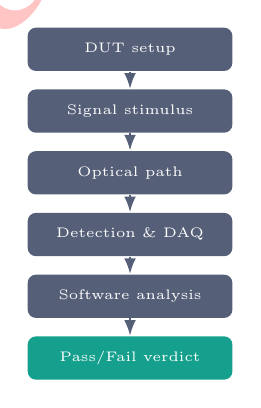
\begin{tikzpicture}[node distance=2.2mm, every node/.style={oblk,fill=islcslate,minimum width=2.6cm,minimum height=0.55cm,font=\tiny}]
            \node(a){DUT setup};
            \node[below=of a](b){Signal stimulus};
            \node[below=of b](c){Optical path};
            \node[below=of c](d){Detection \& DAQ};
            \node[below=of d](e){Software analysis};
            \node[below=of e,fill=islcteal](f){Pass/Fail verdict};
            \draw[oarr](a)--(b);\draw[oarr](b)--(c);\draw[oarr](c)--(d);\draw[oarr](d)--(e);\draw[oarr](e)--(f);
        \end{tikzpicture}
    \end{columns}
\end{frame}

\begin{frame}[allowframebreaks=1.2]{Hardware: bench, Tx \& Rx instruments}
    \textbf{Optical bench}
    \begin{itemize}\footnotesize
        \si Active-pneumatic isolation table (Newport RS2000/TMC); 6-DOF kinematic mounts (sub-$\mu$rad).
        \si 2-axis piezo mirror (PI S-330) emulates jitter; Galilean beam expander; PBS + waveplates.
        \si \key{Fizeau interferometer} ($\lambda/100$), \key{Shack--Hartmann WFS} (150 lenslets), beam profiler ($M^2$), calibrated power meter + ND set; SMF-28 delay-line emulator.
    \end{itemize}
    \framebreak
    \textbf{Tx-chain instruments}
    \begin{itemize}\footnotesize
        \si Tunable laser source (Keysight 81600B / Santec TSL-710), 1480--1640\,nm, $<$100\,kHz.
        \si Optical spectrum analyzer (Yokogawa AQ6370D), 0.02\,nm res, $>$70\,dB --- OSNR/ASE.
        \si VNA (Keysight E5063A) for MZM EO bandwidth ($>$40\,GHz); AWG (Keysight M8195A) PRBS-31 / IQ drive.
    \end{itemize}
    \framebreak
    \textbf{Rx-chain instruments}
    \begin{itemize}\footnotesize
        \si APD characterization: Keithley 2400 SMU bias, responsivity, $-3$\,dB BW, NEP (FEMTO TIA + SR830).
        \si \key{BER \& sensitivity}: BERT (Anritsu MP1800A), VOA sweep ($-25$ to $-55$\,dBm), CDR, 80\,GHz sampling scope --- read sensitivity at BER $=10^{-12}$.
    \end{itemize}
\end{frame}

\begin{frame}[allowframebreaks=1.2]{PAT test, DAQ/FPGA \& software stack}
    \textbf{PAT test hardware}
    \begin{itemize}\footnotesize
        \si Jitter emulator (PI S-330.2SL + AWG, 0--2\,mrad, 1--1000\,Hz); 4-QD (Hamamatsu G6849, $>$100\,kHz).
        \si FSM + E-727 driver ($\pm10$\,V $\to\pm5$\,mrad, $<$0.1\,$\mu$rad); coarse gimbal; CMOS InGaAs camera.
        \si \key{Real-time controller}: NI cRIO-9049 (Xilinx Kintex-7) running PID + notch + Kalman at 50--100\,kHz.
    \end{itemize}
    \framebreak
    \textbf{FPGA control loop (100\,kHz, $\sim$10\,$\mu$s budget)}
    \begin{enumerate}[label=\arabic*.]\scriptsize
        \item ADC read 4-QD $\to$ centroid error (10\,$\mu$s)
        \item Bandpass error filter, 100--800\,Hz (1\,$\mu$s)
        \item Velocity-form PID (2\,$\mu$s)
        \item IIR notch sections at $\omega_n$, $f_{RW}$, $2f_{RW}$, $3f_{RW}$ (2\,$\mu$s)
        \item Kalman predict + disturbance feed-forward (3\,$\mu$s)
        \item DAC write to FSM, saturated at $\pm9.5$\,V (2\,$\mu$s)
    \end{enumerate}
    \framebreak
    \textbf{Software layers}
    \begin{itemize}\footnotesize
        \si L5 Analysis: Python/MATLAB --- NumPy, SciPy, matplotlib, pandas.
        \si L4 Orchestration: LabVIEW TestStand / pytest, SCPI drivers, CI.
        \si L3 Real-time: LabVIEW RT / Simulink RT --- PAT state machine, Kalman.
        \si L2 FPGA: VHDL/Vivado --- PID + notch, 100\,kHz.
        \si L1 Drivers: NI-VISA / NI-DAQmx, SCPI over GPIB/USB/LAN.
    \end{itemize}
\end{frame}

\begin{frame}{Integrated hardware + software test chain}
    \begin{center}
    \scriptsize
    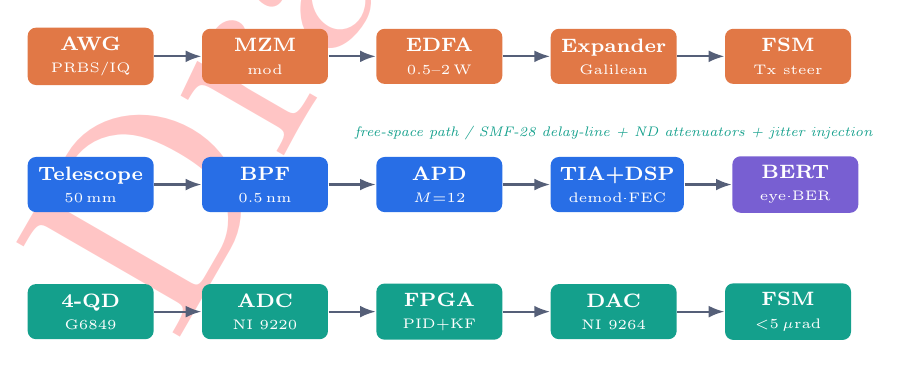
\begin{tikzpicture}[node distance=2.5mm and 6mm]
        % Tx row
        \node[oblk,fill=islcorange,minimum width=1.6cm,minimum height=0.7cm](awg){\textbf{AWG}\\\tiny PRBS/IQ};
        \node[oblk,fill=islcorange,minimum width=1.6cm,minimum height=0.7cm,right=of awg](mzm){\textbf{MZM}\\\tiny mod};
        \node[oblk,fill=islcorange,minimum width=1.6cm,minimum height=0.7cm,right=of mzm](edfa){\textbf{EDFA}\\\tiny 0.5--2\,W};
        \node[oblk,fill=islcorange,minimum width=1.6cm,minimum height=0.7cm,right=of edfa](be){\textbf{Expander}\\\tiny Galilean};
        \node[oblk,fill=islcorange,minimum width=1.6cm,minimum height=0.7cm,right=of be](fsm1){\textbf{FSM}\\\tiny Tx steer};
        \draw[oarr](awg)--(mzm);\draw[oarr](mzm)--(edfa);\draw[oarr](edfa)--(be);\draw[oarr](be)--(fsm1);
        % channel
        \node[below=4mm of be, text=islcteal, font=\tiny\itshape](ch){free-space path / SMF-28 delay-line + ND attenuators + jitter injection};
        % Rx row
        \node[oblk,fill=islcblue,minimum width=1.6cm,minimum height=0.7cm,below=9mm of awg](tele){\textbf{Telescope}\\\tiny 50\,mm};
        \node[oblk,fill=islcblue,minimum width=1.6cm,minimum height=0.7cm,right=of tele](bpf){\textbf{BPF}\\\tiny 0.5\,nm};
        \node[oblk,fill=islcblue,minimum width=1.6cm,minimum height=0.7cm,right=of bpf](apd){\textbf{APD}\\\tiny $M{=}12$};
        \node[oblk,fill=islcblue,minimum width=1.6cm,minimum height=0.7cm,right=of apd](tia){\textbf{TIA+DSP}\\\tiny demod·FEC};
        \node[oblk,fill=islcpurple,minimum width=1.6cm,minimum height=0.7cm,right=of tia](bert){\textbf{BERT}\\\tiny eye·BER};
        \draw[oarr](tele)--(bpf);\draw[oarr](bpf)--(apd);\draw[oarr](apd)--(tia);\draw[oarr](tia)--(bert);
        % PAT row
        \node[oblk,fill=islcteal,minimum width=1.6cm,minimum height=0.7cm,below=9mm of tele](qd){\textbf{4-QD}\\\tiny G6849};
        \node[oblk,fill=islcteal,minimum width=1.6cm,minimum height=0.7cm,right=of qd](adc){\textbf{ADC}\\\tiny NI 9220};
        \node[oblk,fill=islcteal,minimum width=1.6cm,minimum height=0.7cm,right=of adc](fpga){\textbf{FPGA}\\\tiny PID+KF};
        \node[oblk,fill=islcteal,minimum width=1.6cm,minimum height=0.7cm,right=of fpga](dac){\textbf{DAC}\\\tiny NI 9264};
        \node[oblk,fill=islcteal,minimum width=1.6cm,minimum height=0.7cm,right=of dac](fsm2){\textbf{FSM}\\\tiny $<$5\,$\mu$rad};
        \draw[oarr](qd)--(adc);\draw[oarr](adc)--(fpga);\draw[oarr](fpga)--(dac);\draw[oarr](dac)--(fsm2);
    \end{tikzpicture}
    \end{center}
    \footnotesize Top: transmit side. Middle: emulated channel. Bottom: closed PAT tracking loop.
\end{frame}

\begin{frame}{Key measurement sequences \& acceptance criteria}
    \footnotesize
    \begin{columns}[T]
    \column{0.33\textwidth}
        \textbf{WFE \& Strehl}
        \begin{itemize}\scriptsize
            \si SH-WFS, 100 frames, Zernike Z4--Z37
            \si RSS WFE; Strehl via Mar\'echal
        \end{itemize}
        \textcolor{islcteal}{$\checkmark$ RSS WFE $<$30\,nm, $S>0.80$}
    \column{0.33\textwidth}
        \textbf{FSM loop closure}
        \begin{itemize}\scriptsize
            \si Swept-sine $\to$ $H(f)$, fit $\omega_n,\zeta$
            \si PID+notch, inject 60/120/180\,Hz
        \end{itemize}
        \textcolor{islcteal}{$\checkmark$ RMS $<$5\,$\mu$rad, BW $>$500\,Hz}
    \column{0.33\textwidth}
        \textbf{BER waterfall}
        \begin{itemize}\scriptsize
            \si Sweep VOA, fit $0.5\,\mathrm{erfc}(Q/\sqrt2)$
            \si Margin $\ge3$\,dB
        \end{itemize}
        \textcolor{islcteal}{$\checkmark$ $\le-35$\,dBm @ 10G, $10^{-12}$}
    \end{columns}
    \vspace{2mm}
    \begin{block}{Environmental qualification}
    \scriptsize TVAC ($<10^{-6}$\,mbar, $-40$ to $+70^\circ$C, in-situ WFS) --- WFE RSS $<$35\,nm, $S>0.78$. \quad
    Vibration (GEVS-7000A, 14.1\,$g_{rms}$) + 3000\,g shock. \quad Co-60 TID (10--50\,krad Si) on EDFA fiber \& APD.
    \end{block}
\end{frame}

%===============================================================================================
\section{Flown Hardware \& Conclusion}

\begin{frame}{Reference CubeSat-class terminals}
    \begin{columns}[T]
    \column{0.5\textwidth}
        \begin{block}{CLICK-B/C~\cite{cahoy2020click}}
        \footnotesize MIT / UF / NASA
        \begin{itemize}\scriptsize
            \si Two 3U CubeSats; sub-2U terminals
            \si 20\,Mbps full-duplex, 25--580\,km
            \si 1537/1563\,nm, $\sim$200\,mW, direct detection
            \si MEMS fast-steering mirror \& ranging
        \end{itemize}
        \end{block}
    \column{0.5\textwidth}
        \begin{block}{TBIRD~\cite{robinson2018tbird,schieler2023tbird}}
        \footnotesize MIT Lincoln Laboratory
        \begin{itemize}\scriptsize
            \si 3U payload on a 6U bus
            \si 100 / 200\,Gbps downlink to ground
            \si Coherent fiber-coupled COTS transceivers
            \si ARQ error-free delivery --- up to 4.8\,TB/pass
        \end{itemize}
        \end{block}
    \end{columns}
    \vspace{2mm}
    \centering\footnotesize Interoperability is converging on the SDA \key{Optical Communications Terminal (OCT)} standard~\cite{sda2022oct}.
\end{frame}

\begin{frame}{Key takeaways}
    \begin{itemize}
        \ai OISL is the \key{laser backbone} of modern constellations --- vast gain and bandwidth from a tiny aperture~\cite{kaushal2017optical,toyoshima2021trends}.
        \ai The narrow beam makes \hi{pointing, not photons,} the dominant engineering risk.
        \ai The link budget governs everything: \key{$P_{rx}\propto D^{4}$} --- aperture is the highest-leverage variable.
        \ai Point-ahead, Tx/Rx isolation and FSM jitter rejection are the defining sub-problems; the \key{FSM tracking loop} (PID + notch, $>$500\,Hz, Kalman) is the critical control subsystem.
        \ai CubeSat-scale OISL ($<$50\,mm, $<$1\,W, 1U) enables \key{Gbps+ at $<$800\,km} --- feasible today. Frontiers: MEMS FSM, photonic-IC transceivers, coherent QPSK.
    \end{itemize}
\end{frame}

%-----------------------------------------------------------------------------------------------
\begin{frame}{}
    \centering
    \vfill
    {\fontsize{22}{26}\selectfont \textcolor{islcteal}{\textbf{Thank you}}}\\[4mm]
    {\large Questions \& discussion}
    \vfill
\end{frame}
%-----------------------------------------------------------------------------------------------
\begin{frame}[allowframebreaks=0.9]{References}
    \bibliographystyle{model1-num-names}
    \bibliography{cas-refs}
    \framebreak
\end{frame}
%-----------------------------------------------------------------------------------------------
\end{document}



% These "\usepackage{}" commands import packages into the LaTeX document.
\usepackage[english]{babel}
\usepackage[light,math]{anttor}
\usepackage{graphicx,graphbox}
\usepackage{parskip}
\usepackage{amsmath}
\usepackage{caption}
\usepackage{subcaption}
\usepackage{background}
\usepackage{xcolor}

\usepackage[skins, theorems]{tcolorbox}
\usepackage{pifont}
\usepackage{amssymb,enumitem}
\usepackage{indentfirst}
\usepackage{tabularray}
\usepackage{hyperref}
\usepackage{cleveref}
\usepackage{array}
\usepackage{multirow}
\setbeamertemplate{caption}[numbered]
\usepackage[square,numbers,sort&compress]{natbib}
\renewcommand{\bibsection}{\subsubsection*{\bibname}}
\setbeamertemplate{frametitle continuation}[from second][(contd.)]
\usepackage{setspace}
\onehalfspacing

% Extra TikZ libraries for the block diagrams (tikz + positioning come from the class)
\usetikzlibrary{arrows.meta,positioning,shapes.geometric,fit,backgrounds,calc}

\usetheme{Madrid}
\usecolortheme{default}
\hypersetup{
    colorlinks=true,
    linkcolor=cyan,
    urlcolor=cyan,
    citecolor=cyan,
}

%------------------------------------------------------------
% ISLC colour palette (complements the kaist-* colours from the class)
\definecolor{islcteal}{RGB}{20,160,140}
\definecolor{islcblue}{RGB}{40,110,230}
\definecolor{islcorange}{RGB}{225,120,70}
\definecolor{islcslate}{RGB}{85,95,120}
\definecolor{islcpurple}{RGB}{120,95,210}

% Shorthand bullets and highlight macros to keep the body readable
\newcommand{\ai}{\item[\textcolor{islcteal}{\ding{228}}]}      % primary bullet
\newcommand{\si}{\item[\textcolor{islcorange}{\ding{167}}]}    % sub bullet
\newcommand{\hi}[1]{\textcolor{islcorange}{\textbf{#1}}}       % inline highlight
\newcommand{\key}[1]{\textcolor{islcblue}{\textbf{#1}}}        % inline key term

% Generic TikZ block styles for the architecture / chain diagrams
\tikzset{
  oblk/.style={rectangle, rounded corners=3pt, draw=none, text=white,
               align=center, font=\scriptsize, minimum width=2.6cm, minimum height=1.15cm},
  oarr/.style={-{Latex[length=2mm]}, thick, islcslate},
}

%------------------------------------------------------------
% Title-page information
\title[ISLC for CubeSats] %optional
{Inter-Satellite Laser Communication for CubeSat Platforms}

\subtitle{Optical terminal architecture, design \& experimental setup}

\author[Dinaol Gadisa] % (optional)
{Dinaol Gadisa\inst{1} \and Hyochoong Bang\inst{1}}

\institute[ASCL] % (optional)
{
  \inst{1}%
  Aerospace System and Control Lab, Department of Aerospace Engineering, KAIST\\
}

\date[ASCL-P2026] % (optional)
{ISLC research report, June 2026}

%End of title-page configuration block
%------------------------------------------------------------

% Put a table of contents at the start of every section
\AtBeginSection[]
{
  \begin{frame}
    \frametitle{Table of Contents}
    \tableofcontents[currentsection]
  \end{frame}
}

\renewcommand{\titlelogo}{logo/ascl logo.svg}
\renewcommand{\slidelogo}{logo/ascl logo.svg}
% If \includesvg is unavailable, drop the extension and use a raster logo instead:
% \renewcommand{\titlelogo}{logo/ascl logo}
% \renewcommand{\slidelogo}{logo/ascl logo}

\backgroundsetup{
  scale=0.6,
  angle=0,
  opacity=0.02,
  contents={
    
\includegraphics[width=\textwidth,height=\textwidth]{figs/download.png}}
}

\renewcommand{\slidefoot}{Dinaol Gadisa}
%-----------------------------------------------------------------------------------------------
\begin{document}

\frame{\titlepage}

%===============================================================================================
\section{Introduction \& Motivation}

\begin{frame}[t,allowframebreaks=1.2]{Why optical inter-satellite links?}
    \begin{itemize}
        \ai Inter-satellite laser communication (\hi{ISLC}, also \hi{OISL}) links satellites \key{directly} to one another with laser beams instead of routing every bit down to the ground and back up~\cite{kaushal2017optical,sodnik2010optical}.
        \ai The carrier is a near-infrared laser --- typically \key{1550\,nm} ($\sim$193\,THz) --- inherited from the fiber-telecom ecosystem.
        \ai Chained across a constellation, the links form a \key{low-latency optical mesh} that moves data in orbit --- the in-space backbone of Starlink, Kuiper and the SDA transport layer~\cite{chaudhry2021free,sda2022oct}.
    \end{itemize}
    \framebreak
    \begin{block}{Optical vs.\ RF --- why lasers win in space~\cite{kaushal2017optical}}
    \centering\footnotesize
    \begin{tabular}{l l l}
        \hline
        \textbf{Parameter} & \textbf{Ka-band RF} & \textbf{OISL @ 1550\,nm}\\
        \hline
        Data rate      & 100--600\,Mbps   & 1--100\,Gbps\\
        Carrier        & 26--40\,GHz      & $\sim$193\,THz\\
        Beam divergence& $\sim0.5$--$2^\circ$ & $\sim$10--100\,$\mu$rad\\
        Aperture       & 200--600\,mm     & 30--100\,mm\\
        Licensing      & \textcolor{red}{Required} & \textcolor{islcteal}{None (LPI/LPD)}\\
        \hline
    \end{tabular}
    \end{block}
    \begin{itemize}
        \ai \hi{The catch:} a tens-of-$\mu$rad beam must be pointed to a few $\mu$rad across thousands of km --- \key{pointing, not photons, is the hard problem}.
    \end{itemize}
\end{frame}

\begin{frame}{Advantages of OISL}
    \begin{columns}[T]
    \column{0.5\textwidth}
        \begin{itemize}
            \ai \hi{10--100$\times$} higher data rate than Ka-band RF
            \ai \hi{$\sim$10\,$\mu$rad} beam divergence (vs.\ $\sim1^\circ$ for RF)
            \ai \hi{No ITU} frequency licensing required
            \ai \hi{$<$50\%} mass \& aperture vs.\ equivalent RF
        \end{itemize}
    \column{0.5\textwidth}
        \begin{block}{CubeSat relevance~\cite{toyoshima2021trends,cahoy2020click}}
        A 50\,mm-aperture OISL achieves \key{Gbps at 500\,km} in a $\sim$0.5U volume --- impossible with RF in the same form factor.
        \end{block}
    \end{columns}
\end{frame}

%===============================================================================================
\section{Link Fundamentals}

\begin{frame}[allowframebreaks=1.2]{The link in one equation}
    \begin{itemize}
        \ai The received power follows the free-space optical link equation~\cite{hemmati2009near,caplan2007laser}:
    \end{itemize}
    \begin{equation*}
        \tcbhighmath[boxrule=1pt,arc=2pt,colback=islcteal!4,colframe=islcblue,drop fuzzy shadow=islcslate]{%
        P_{rx} = P_{tx}\, G_{tx}\, \left(\frac{\lambda}{4\pi R}\right)^{2} G_{rx}\, L_{point}\, L_{impl}}
    \end{equation*}
    \begin{itemize}
        \si \hi{Aperture gain} $G = (\pi D/\lambda)^2 \approx +100$\,dB for a diffraction-limited 5\,cm telescope.
        \si \hi{Free-space loss} $(\lambda/4\pi R)^2 \approx -262$\,dB over 1500\,km at 1550\,nm.
        \si \hi{Pointing loss} $\propto e^{-2(\theta/\theta_0)^2}$ --- $\tfrac13$ of a beamwidth off $\approx$ 1\,dB lost.
    \end{itemize}
    \framebreak
    \begin{itemize}
        \ai Two competing quantities set everything: \key{antenna gain} and \key{beam divergence}
        \begin{equation*}
            G = \left(\frac{\pi D}{\lambda}\right)^{2}, \qquad \theta \approx \frac{\lambda}{D}\approx\frac{\lambda}{\pi w_0}.
        \end{equation*}
        \ai Enormous gains fight an enormous path loss; \key{sensitivity} is then set by \hi{photons/bit}:
        \begin{equation*}
            P_{req} = \left(\frac{\text{photons}}{\text{bit}}\right)\frac{hc}{\lambda}\,R_b .
        \end{equation*}
        \si OOK $\approx$ tens, DPSK $\approx 38$, coherent $\approx 9$ photons/bit at BER $10^{-9}$~\cite{caplan2007laser}.
    \end{itemize}
\end{frame}

%===============================================================================================
\section{Optical Terminal Architecture}

\begin{frame}{Terminal architecture at a glance}
    \begin{center}
    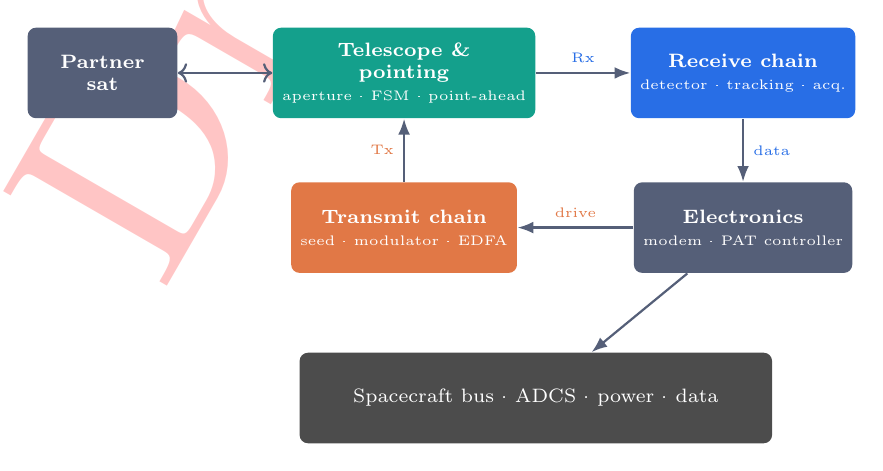
\begin{tikzpicture}[node distance=8mm and 12mm]
        \node[oblk, fill=islcslate, minimum width=1.9cm](sat){\textbf{Partner}\\\textbf{sat}};
        \node[oblk, fill=islcteal, right=of sat](tel){\textbf{Telescope \&}\\\textbf{pointing}\\\tiny aperture · FSM · point-ahead};
        \node[oblk, fill=islcblue, right=of tel](rx){\textbf{Receive chain}\\\tiny detector · tracking · acq.};
        \node[oblk, fill=islcorange, below=of tel](tx){\textbf{Transmit chain}\\\tiny seed · modulator · EDFA};
        \node[oblk, fill=islcslate, below=of rx](el){\textbf{Electronics}\\\tiny modem · PAT controller};
        \node[oblk, fill=black!70, minimum width=6cm, below=10mm of el.south -| tel.east](bus){\scriptsize Spacecraft bus · ADCS · power · data};

        \draw[oarr,<->](sat)--(tel);
        \draw[oarr](tel)-- node[above,font=\tiny,text=islcblue]{Rx} (rx);
        \draw[oarr](rx)-- node[right,font=\tiny,text=islcblue]{data} (el);
        \draw[oarr](el)-- node[above,font=\tiny,text=islcorange]{drive} (tx);
        \draw[oarr](tx.north)-- node[left,font=\tiny,text=islcorange]{Tx} (tel.south);
        \draw[oarr](el)--(bus);
    \end{tikzpicture}
    \end{center}
    \footnotesize Four blocks around \key{one shared aperture} that transmits watts, receives nanowatts and steers to microradians~\cite{sodnik2010optical}.
\end{frame}

\begin{frame}[allowframebreaks=1.2]{Aperture, transmit \& receive chains}
    \begin{itemize}
        \ai \hi{Aperture \& telescope.} A single aperture is shared by Tx and Rx to save mass; the hard part is \key{Tx/Rx isolation} --- $\sim$1\,W out vs.\ $\sim$10\,nW in is an 80--100\,dB dynamic range, won by wavelength offset (e.g.\ 1537/1563\,nm), polarization, or time-division.
    \end{itemize}
    \framebreak
    \textbf{Transmit chain} --- a fiber-laser (MOPA) stack:
    \begin{center}
    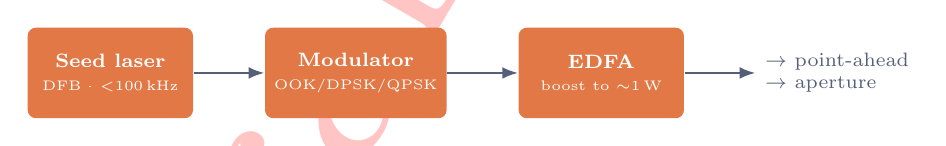
\begin{tikzpicture}[node distance=5mm and 9mm]
        \node[oblk, fill=islcorange, minimum width=2.1cm](seed){\textbf{Seed laser}\\\tiny DFB · $<$100\,kHz};
        \node[oblk, fill=islcorange, minimum width=2.1cm, right=of seed](mod){\textbf{Modulator}\\\tiny OOK/DPSK/QPSK};
        \node[oblk, fill=islcorange, minimum width=2.1cm, right=of mod](edfa){\textbf{EDFA}\\\tiny boost to $\sim$1\,W};
        \node[right=of edfa, font=\scriptsize, align=left, text=islcslate](out){$\rightarrow$ point-ahead\\$\rightarrow$ aperture};
        \draw[oarr](seed)--(mod);\draw[oarr](mod)--(edfa);\draw[oarr](edfa)--(out);
    \end{tikzpicture}
    \end{center}
    \framebreak
    \textbf{Receive chain} --- the incoming beam is tapped three ways:
    \begin{center}
    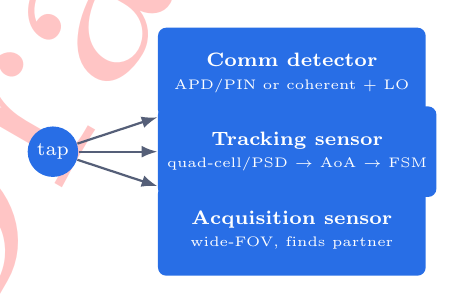
\begin{tikzpicture}[node distance=4mm and 10mm]
        \node[circle,fill=islcblue,text=white,font=\scriptsize,inner sep=2pt](tap){tap};
        \node[oblk, fill=islcblue, right=of tap, yshift=10mm, minimum width=3.4cm](comm){\textbf{Comm detector}\\\tiny APD/PIN or coherent + LO};
        \node[oblk, fill=islcblue, right=of tap, minimum width=3.4cm](trk){\textbf{Tracking sensor}\\\tiny quad-cell/PSD $\to$ AoA $\to$ FSM};
        \node[oblk, fill=islcblue, right=of tap, yshift=-10mm, minimum width=3.4cm](acq){\textbf{Acquisition sensor}\\\tiny wide-FOV, finds partner};
        \draw[oarr](tap)--(comm);\draw[oarr](tap)--(trk);\draw[oarr](tap)--(acq);
    \end{tikzpicture}
    \end{center}
    \framebreak
    \begin{itemize}
        \ai \hi{Electronics \& control.} The \key{modem} runs FEC (LDPC), framing and an ARQ retransmit layer for error-free delivery through fades; the \key{PAT controller} runs the nested acquisition/tracking loops, computes point-ahead and closes the FSM loop.
        \ai It also handles \key{Doppler}: at 1550\,nm a 15\,km/s closing rate shifts the carrier by $\sim$10\,GHz, tracked by an AFC loop on coherent systems.
    \end{itemize}
\end{frame}

%===============================================================================================
\section{Optical Components}

\begin{frame}[allowframebreaks=1.2]{Laser source \& modulation}
    \begin{columns}[T]
    \column{0.52\textwidth}
        \textbf{MOPA laser source}
        \begin{itemize}\footnotesize
            \si $\lambda = 1550$\,nm (eye-safe, EDFA band)
            \si DFB seed, linewidth $<100$\,kHz
            \si 10--40\,mW seed $\to$ 0.5--5\,W via EDFA
            \si Linear polarization (MZM requirement)
            \si RIN $< -150$\,dB/Hz; rad-hard Er-fiber
        \end{itemize}
    \column{0.48\textwidth}
        \textbf{Modulation formats}~\cite{caplan2007laser}
        \begin{itemize}\footnotesize
            \si \key{OOK}: simple, $\sim-28$\,dBm @ 10G
            \si \key{DPSK}: +3\,dB, $\sim-31$\,dBm @ 10G
            \si \key{QPSK}: coherent, $\sim-35$\,dBm @ 10G
        \end{itemize}
    \end{columns}
    \vspace{2mm}
    \begin{block}{Doppler challenge @ 1550\,nm}
    Two LEO satellites at 7.5\,km/s $\Rightarrow$ $\Delta f = f\,v/c \approx 5$\,GHz Doppler shift $\Rightarrow$ requires optical pre-compensation / AFC in the PAT loop.
    \end{block}
\end{frame}

\begin{frame}[allowframebreaks=1.2]{Beam expander, FSM \& detector}
    \begin{columns}[T]
    \column{0.5\textwidth}
        \textbf{Beam expander (Tx telescope)}
        \begin{itemize}\footnotesize
            \si Galilean afocal (no focus $\to$ no air breakdown)
            \si $D = 30$--80\,mm; CubeSat $\sim$50\,mm
            \si $\theta \approx \lambda/(\pi w_0)\approx40\,\mu$rad @ 50\,mm
            \si $\sim$20\,m footprint @ 500\,km (vs.\ 4\,km Ka)
            \si Strehl $>0.8 \Rightarrow$ WFE $<\lambda/14=111$\,nm RMS
        \end{itemize}
    \column{0.5\textwidth}
        \textbf{Fine steering mirror (FSM)}
        \begin{itemize}\footnotesize
            \si 15--30\,mm clear aperture, PZT or VCA
            \si Range $\pm1$--5\,mrad, resolution $<1\,\mu$rad
            \si Bandwidth $>500$\,Hz to reject RW harmonics
            \si Shared by Tx pointing \& PAT correction
        \end{itemize}
    \end{columns}
    \framebreak
    \begin{block}{Photodetectors}
    \footnotesize
    \key{InGaAs APD} (workhorse, LEO--LEO): gain $M=5$--20, $-30$ to $-35$\,dBm @ 10G, room temperature, 900--1650\,nm. \quad
    \key{SNSPD} (deep-space, photon-starved): single-photon, $>$90\% efficiency, $<$50\,ps jitter --- flown on NASA LLCD~\cite{boroson2014llcd}.
    \end{block}
    \begin{center}\scriptsize
    
\begin{tikzpicture}[node distance=3mm and 6mm]
        \node[oblk,fill=islcteal,minimum width=1.7cm](t){\textbf{Cassegrain}\\\tiny 50--100\,mm};
        \node[oblk,fill=islcteal,minimum width=1.7cm,right=of t](f){\textbf{BPF}\\\tiny 0.3--1\,nm};
        \node[oblk,fill=islcteal,minimum width=1.7cm,right=of f](fo){\textbf{Focus}\\\tiny f/4--f/8};
        \node[oblk,fill=islcteal,minimum width=1.7cm,right=of fo](apd){\textbf{APD}\\\tiny $M{=}10$--15};
        \node[oblk,fill=islcteal,minimum width=1.7cm,right=of apd](dsp){\textbf{TIA+DSP}\\\tiny demod·FEC};
        \draw[oarr](t)--(f);\draw[oarr](f)--(fo);\draw[oarr](fo)--(apd);\draw[oarr](apd)--(dsp);
    \end{tikzpicture}
    \end{center}
    \centering\footnotesize Complete receive chain. \quad Key coupling: $\theta\propto\lambda/D$ --- larger aperture $=$ narrower beam $=$ higher gain $=$ tighter pointing requirement.
\end{frame}

%===============================================================================================
\section{Pointing, Acquisition \& Tracking}

\begin{frame}[allowframebreaks=1.2]{Point-ahead \& acquisition}
    \begin{itemize}
        \ai Light takes time to cross the link and both satellites move --- you transmit toward where the partner \key{WILL be} while its beam arrives from where it \key{WAS}~\cite{kaushal2017optical}.
        \ai The lead angle is
        \begin{equation*}
            \alpha_{PA}\approx \frac{2v_\perp}{c}.
        \end{equation*}
        \si Cross-plane LEO: $v_\perp$ up to $\sim$15\,km/s gives $\sim$100\,$\mu$rad --- comparable to the whole beamwidth, so a dedicated actuator is required.
        \si Same-plane crosslinks move together: point-ahead nearly vanishes.
    \end{itemize}
    \framebreak
    \textbf{From blind to locked --- 3-stage PAT}
    \begin{center}
    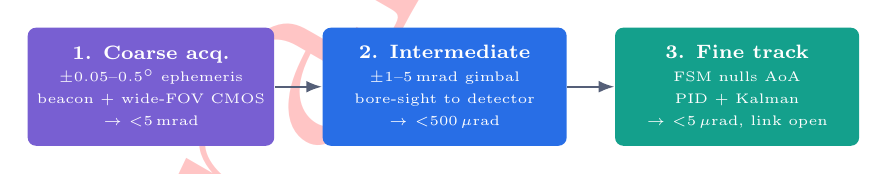
\begin{tikzpicture}[node distance=6mm]
        \node[oblk,fill=islcpurple,minimum width=3.1cm,minimum height=1.5cm](s1){\textbf{1. Coarse acq.}\\\tiny $\pm0.05$--$0.5^\circ$ ephemeris\\\tiny beacon + wide-FOV CMOS\\\tiny $\to$ $<$5\,mrad};
        \node[oblk,fill=islcblue,minimum width=3.1cm,minimum height=1.5cm,right=of s1](s2){\textbf{2. Intermediate}\\\tiny $\pm1$--5\,mrad gimbal\\\tiny bore-sight to detector\\\tiny $\to$ $<$500\,$\mu$rad};
        \node[oblk,fill=islcteal,minimum width=3.1cm,minimum height=1.5cm,right=of s2](s3){\textbf{3. Fine track}\\\tiny FSM nulls AoA\\\tiny PID + Kalman\\\tiny $\to$ $<$5\,$\mu$rad, link open};
        \draw[oarr](s1)--(s2);\draw[oarr](s2)--(s3);
    \end{tikzpicture}
    \end{center}
\end{frame}

\begin{frame}[allowframebreaks=1.2]{FSM tracking-loop design}
    \begin{itemize}
        \ai \hi{Plant} --- a lightly damped resonant mirror:
        \begin{equation*}
            P(s)=\frac{K_{act}\,\omega_n^{2}}{s^{2}+2\zeta\omega_n s+\omega_n^{2}},\quad
            \begin{aligned}
            &\omega_n = 2\pi\!\times\!500\text{--}2000\ \text{rad/s}\\
            &\zeta = 0.01\text{--}0.05,\ K_{act}=10\text{--}50\,\mu\text{rad/V}
            \end{aligned}
        \end{equation*}
        \ai \hi{Controller} $C(s)=$ PID $\times$ notches, crossover $f_c\approx300$\,Hz, phase margin $\ge45^\circ$, gain margin $\ge6$\,dB. The notch
        \begin{equation*}
            N(s)=\frac{s^{2}+2\zeta_z\omega_n s+\omega_n^{2}}{s^{2}+2\zeta_p\omega_n s+\omega_n^{2}},\quad \zeta_z\!=\!0.001,\ \zeta_p\!=\!0.3\text{--}0.5
        \end{equation*}
        places a deep null at each mechanical / reaction-wheel resonance.
    \end{itemize}
    \framebreak
    \begin{itemize}
        \ai \hi{Sensing.} 4-quadrant detector (up to 100\,kHz, $\pm$20\% spot linear range) gives the centroid error
        \begin{equation*}
            \varepsilon_x=\frac{(A+B)-(C+D)}{A+B+C+D}.
        \end{equation*}
        \ai \hi{Kalman estimator.} State $x=[\theta,\dot\theta,d_{dist}]^\mathsf{T}$ with update
        \begin{equation*}
            K_k = P_k^{-}H^\mathsf{T}\!\left(HP_k^{-}H^\mathsf{T}+R\right)^{-1},\quad R\approx(0.5\,\mu\text{rad})^2 .
        \end{equation*}
        \si Disturbance feed-forward $u_{ff}=-K_{ff}\hat d$ cancels reaction-wheel harmonics by \key{15--25\,dB} vs.\ PID alone.
    \end{itemize}
\end{frame}

%===============================================================================================
\section{Wavefront Error Budget}

\begin{frame}[allowframebreaks=1.2]{From surface to Strehl}
    \begin{itemize}
        \ai Wavefront quality maps to coupling efficiency through the \key{Mar\'echal approximation}~\cite{born1999principles}:
        \begin{equation*}
            \tcbhighmath[boxrule=1pt,arc=2pt,colback=islcteal!4,colframe=islcorange]{%
            S \approx \exp\!\left[-\left(\frac{2\pi\sigma}{\lambda}\right)^{2}\right]}
        \end{equation*}
        where $\sigma$ is the RMS wavefront error. Diffraction-limited $\equiv S>0.8$.
    \end{itemize}
    \framebreak
    \begin{block}{Representative WFE budget (RSS)}
    \centering\scriptsize
    \begin{tabular}{l r}
        \hline
        \textbf{Contributor} & \textbf{nm RMS}\\
        \hline
        Primary mirror surface figure & 11\\
        Secondary mirror figure       & 8\\
        Relay lens transmitted WFE    & 6\\
        AR/HR coating micro-roughness & 4\\
        Mirror decenter (assembly)    & 9\\
        Axial despace / focus error   & 7\\
        Thermal gradient deformation  & 12\\
        Mounting stress (flexures)    & 6\\
        Residual vibration post-FSM   & 4\\
        \hline
        \textbf{RSS total} & \textbf{23.7}\\
        \hline
    \end{tabular}
    \end{block}
    \centering Strehl $S\approx0.91 \Rightarrow$ \key{diffraction-limited} (criterion $S>0.8$).
    \framebreak
    \textbf{WFE design process --- requirement to hardware}
    \begin{enumerate}[label=\arabic*.]\footnotesize
        \item System Strehl requirement (from link budget); set target to 70\% of limit for margin.
        \item Zemax sensitivity analysis: $S_{ij}=\partial\text{WFE}_i/\partial\text{DOF}_j$ identifies dominant terms (e.g.\ secondary decenter $\to$ coma).
        \item WFE allocation: invert sensitivities, $\delta_j=\sigma_i/S_{ij}$, iterate to achievable tolerances.
        \item Manufacture \& metrology: Fizeau interferometry ($\lambda/50$), ion-beam polishing.
        \item Space qualification: TVAC, vibration, shock, TID.
        \item End-to-end link test with range-equivalent attenuation.
    \end{enumerate}
\end{frame}

%===============================================================================================
\section{CubeSat Link Budget}

\begin{frame}[allowframebreaks=1.2]{CubeSat OISL trade-space}
    \begin{equation*}
        P_{rx}=P_{tx}\,\eta_{tx}\frac{\pi D_{tx}^{2}}{4\lambda^{2}}\cdot\frac{\pi D_{rx}^{2}}{4R^{2}}\,\eta_{rx}\,L_{point}
    \end{equation*}
    \begin{columns}[T]
    \column{0.55\textwidth}
    \scriptsize
    \begin{tabular}{l r}
        \hline
        \textbf{Term (D=40\,mm, 500\,km)} & \textbf{dB}\\
        \hline
        Tx power (0.5\,W)        & $+27.0$\,dBm\\
        Tx optical eff.\ $\eta_{tx}=0.75$ & $-1.2$\\
        Tx aperture gain         & $+76.8$\\
        Free-space path loss     & $-278.2$\\
        Rx aperture (eff.\ area)  & $+67.2$\\
        Rx optical eff.\ $\eta_{rx}=0.60$ & $-2.2$\\
        Pointing loss            & $-2.0$\\
        \hline
        \textbf{Received power}  & $\mathbf{-112.6}$\,\textbf{dBm}\\
        \hline
    \end{tabular}
    \column{0.45\textwidth}
        \begin{itemize}\footnotesize
            \ai APD sensitivity @ 1\,Gbps: \hi{$-41$\,dBm}
            \ai Link margin: \hi{$+28$\,dB}
            \ai Max data rate at these params: \hi{$\sim$3\,Gbps}
        \end{itemize}
    \end{columns}
    \framebreak
    \begin{block}{The two scaling laws that govern everything}
    \footnotesize
    \key{$P_{rx}\propto D^{4}$} --- both apertures scale received power; doubling $D$ on both sides $=+12$\,dB ($\times16$). \\
    \key{$P_{rx}\propto 1/R^{2}$} --- doubling range costs 6\,dB.
    \end{block}
    \begin{itemize}\footnotesize
        \ai \hi{CubeSat limit:} 1U constrains aperture to $\sim$40--50\,mm $\Rightarrow$ Gbps+ links practical to $<$800\,km with 0.5\,W Tx.
        \ai \hi{Power tradeoff:} an EDFA at 1\,W optical draws $\sim$5--8\,W DC --- 50--80\% of a 10\,W CubeSat budget, the dominant system constraint.
    \end{itemize}
\end{frame}

%===============================================================================================
\section{Experimental Test Setup}

\begin{frame}{Experimental strategy \& test hierarchy}
    \begin{columns}[T]
    \column{0.5\textwidth}
        \begin{itemize}\footnotesize
            \ai \key{Component-level}: characterize each optical element (laser, FSM, detector, telescope) in isolation.
            \ai \key{Subsystem-level}: validate Tx chain, Rx chain and PAT loop independently.
            \ai \key{System-level}: end-to-end link with range-equivalent path loss.
            \ai \key{Environmental}: TVAC, vibration, radiation per ECSS / NASA.
        \end{itemize}
    \column{0.5\textwidth}
        \scriptsize
        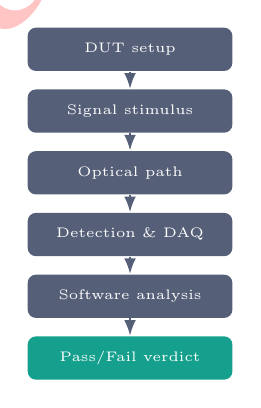
\begin{tikzpicture}[node distance=2.2mm, every node/.style={oblk,fill=islcslate,minimum width=2.6cm,minimum height=0.55cm,font=\tiny}]
            \node(a){DUT setup};
            \node[below=of a](b){Signal stimulus};
            \node[below=of b](c){Optical path};
            \node[below=of c](d){Detection \& DAQ};
            \node[below=of d](e){Software analysis};
            \node[below=of e,fill=islcteal](f){Pass/Fail verdict};
            \draw[oarr](a)--(b);\draw[oarr](b)--(c);\draw[oarr](c)--(d);\draw[oarr](d)--(e);\draw[oarr](e)--(f);
        \end{tikzpicture}
    \end{columns}
\end{frame}

\begin{frame}[allowframebreaks=1.2]{Hardware: bench, Tx \& Rx instruments}
    \textbf{Optical bench}
    \begin{itemize}\footnotesize
        \si Active-pneumatic isolation table (Newport RS2000/TMC); 6-DOF kinematic mounts (sub-$\mu$rad).
        \si 2-axis piezo mirror (PI S-330) emulates jitter; Galilean beam expander; PBS + waveplates.
        \si \key{Fizeau interferometer} ($\lambda/100$), \key{Shack--Hartmann WFS} (150 lenslets), beam profiler ($M^2$), calibrated power meter + ND set; SMF-28 delay-line emulator.
    \end{itemize}
    \framebreak
    \textbf{Tx-chain instruments}
    \begin{itemize}\footnotesize
        \si Tunable laser source (Keysight 81600B / Santec TSL-710), 1480--1640\,nm, $<$100\,kHz.
        \si Optical spectrum analyzer (Yokogawa AQ6370D), 0.02\,nm res, $>$70\,dB --- OSNR/ASE.
        \si VNA (Keysight E5063A) for MZM EO bandwidth ($>$40\,GHz); AWG (Keysight M8195A) PRBS-31 / IQ drive.
    \end{itemize}
    \framebreak
    \textbf{Rx-chain instruments}
    \begin{itemize}\footnotesize
        \si APD characterization: Keithley 2400 SMU bias, responsivity, $-3$\,dB BW, NEP (FEMTO TIA + SR830).
        \si \key{BER \& sensitivity}: BERT (Anritsu MP1800A), VOA sweep ($-25$ to $-55$\,dBm), CDR, 80\,GHz sampling scope --- read sensitivity at BER $=10^{-12}$.
    \end{itemize}
\end{frame}

\begin{frame}[allowframebreaks=1.2]{PAT test, DAQ/FPGA \& software stack}
    \textbf{PAT test hardware}
    \begin{itemize}\footnotesize
        \si Jitter emulator (PI S-330.2SL + AWG, 0--2\,mrad, 1--1000\,Hz); 4-QD (Hamamatsu G6849, $>$100\,kHz).
        \si FSM + E-727 driver ($\pm10$\,V $\to\pm5$\,mrad, $<$0.1\,$\mu$rad); coarse gimbal; CMOS InGaAs camera.
        \si \key{Real-time controller}: NI cRIO-9049 (Xilinx Kintex-7) running PID + notch + Kalman at 50--100\,kHz.
    \end{itemize}
    \framebreak
    \textbf{FPGA control loop (100\,kHz, $\sim$10\,$\mu$s budget)}
    \begin{enumerate}[label=\arabic*.]\scriptsize
        \item ADC read 4-QD $\to$ centroid error (10\,$\mu$s)
        \item Bandpass error filter, 100--800\,Hz (1\,$\mu$s)
        \item Velocity-form PID (2\,$\mu$s)
        \item IIR notch sections at $\omega_n$, $f_{RW}$, $2f_{RW}$, $3f_{RW}$ (2\,$\mu$s)
        \item Kalman predict + disturbance feed-forward (3\,$\mu$s)
        \item DAC write to FSM, saturated at $\pm9.5$\,V (2\,$\mu$s)
    \end{enumerate}
    \framebreak
    \textbf{Software layers}
    \begin{itemize}\footnotesize
        \si L5 Analysis: Python/MATLAB --- NumPy, SciPy, matplotlib, pandas.
        \si L4 Orchestration: LabVIEW TestStand / pytest, SCPI drivers, CI.
        \si L3 Real-time: LabVIEW RT / Simulink RT --- PAT state machine, Kalman.
        \si L2 FPGA: VHDL/Vivado --- PID + notch, 100\,kHz.
        \si L1 Drivers: NI-VISA / NI-DAQmx, SCPI over GPIB/USB/LAN.
    \end{itemize}
\end{frame}

\begin{frame}{Integrated hardware + software test chain}
    \begin{center}
    \scriptsize
    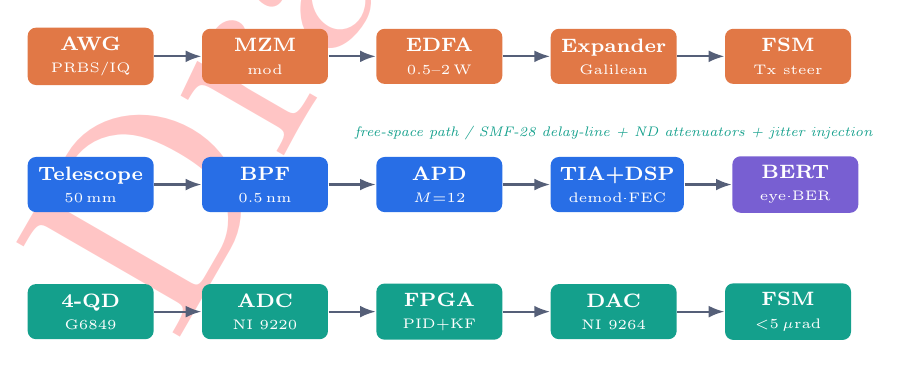
\begin{tikzpicture}[node distance=2.5mm and 6mm]
        % Tx row
        \node[oblk,fill=islcorange,minimum width=1.6cm,minimum height=0.7cm](awg){\textbf{AWG}\\\tiny PRBS/IQ};
        \node[oblk,fill=islcorange,minimum width=1.6cm,minimum height=0.7cm,right=of awg](mzm){\textbf{MZM}\\\tiny mod};
        \node[oblk,fill=islcorange,minimum width=1.6cm,minimum height=0.7cm,right=of mzm](edfa){\textbf{EDFA}\\\tiny 0.5--2\,W};
        \node[oblk,fill=islcorange,minimum width=1.6cm,minimum height=0.7cm,right=of edfa](be){\textbf{Expander}\\\tiny Galilean};
        \node[oblk,fill=islcorange,minimum width=1.6cm,minimum height=0.7cm,right=of be](fsm1){\textbf{FSM}\\\tiny Tx steer};
        \draw[oarr](awg)--(mzm);\draw[oarr](mzm)--(edfa);\draw[oarr](edfa)--(be);\draw[oarr](be)--(fsm1);
        % channel
        \node[below=4mm of be, text=islcteal, font=\tiny\itshape](ch){free-space path / SMF-28 delay-line + ND attenuators + jitter injection};
        % Rx row
        \node[oblk,fill=islcblue,minimum width=1.6cm,minimum height=0.7cm,below=9mm of awg](tele){\textbf{Telescope}\\\tiny 50\,mm};
        \node[oblk,fill=islcblue,minimum width=1.6cm,minimum height=0.7cm,right=of tele](bpf){\textbf{BPF}\\\tiny 0.5\,nm};
        \node[oblk,fill=islcblue,minimum width=1.6cm,minimum height=0.7cm,right=of bpf](apd){\textbf{APD}\\\tiny $M{=}12$};
        \node[oblk,fill=islcblue,minimum width=1.6cm,minimum height=0.7cm,right=of apd](tia){\textbf{TIA+DSP}\\\tiny demod·FEC};
        \node[oblk,fill=islcpurple,minimum width=1.6cm,minimum height=0.7cm,right=of tia](bert){\textbf{BERT}\\\tiny eye·BER};
        \draw[oarr](tele)--(bpf);\draw[oarr](bpf)--(apd);\draw[oarr](apd)--(tia);\draw[oarr](tia)--(bert);
        % PAT row
        \node[oblk,fill=islcteal,minimum width=1.6cm,minimum height=0.7cm,below=9mm of tele](qd){\textbf{4-QD}\\\tiny G6849};
        \node[oblk,fill=islcteal,minimum width=1.6cm,minimum height=0.7cm,right=of qd](adc){\textbf{ADC}\\\tiny NI 9220};
        \node[oblk,fill=islcteal,minimum width=1.6cm,minimum height=0.7cm,right=of adc](fpga){\textbf{FPGA}\\\tiny PID+KF};
        \node[oblk,fill=islcteal,minimum width=1.6cm,minimum height=0.7cm,right=of fpga](dac){\textbf{DAC}\\\tiny NI 9264};
        \node[oblk,fill=islcteal,minimum width=1.6cm,minimum height=0.7cm,right=of dac](fsm2){\textbf{FSM}\\\tiny $<$5\,$\mu$rad};
        \draw[oarr](qd)--(adc);\draw[oarr](adc)--(fpga);\draw[oarr](fpga)--(dac);\draw[oarr](dac)--(fsm2);
    \end{tikzpicture}
    \end{center}
    \footnotesize Top: transmit side. Middle: emulated channel. Bottom: closed PAT tracking loop.
\end{frame}

\begin{frame}{Key measurement sequences \& acceptance criteria}
    \footnotesize
    \begin{columns}[T]
    \column{0.33\textwidth}
        \textbf{WFE \& Strehl}
        \begin{itemize}\scriptsize
            \si SH-WFS, 100 frames, Zernike Z4--Z37
            \si RSS WFE; Strehl via Mar\'echal
        \end{itemize}
        \textcolor{islcteal}{$\checkmark$ RSS WFE $<$30\,nm, $S>0.80$}
    \column{0.33\textwidth}
        \textbf{FSM loop closure}
        \begin{itemize}\scriptsize
            \si Swept-sine $\to$ $H(f)$, fit $\omega_n,\zeta$
            \si PID+notch, inject 60/120/180\,Hz
        \end{itemize}
        \textcolor{islcteal}{$\checkmark$ RMS $<$5\,$\mu$rad, BW $>$500\,Hz}
    \column{0.33\textwidth}
        \textbf{BER waterfall}
        \begin{itemize}\scriptsize
            \si Sweep VOA, fit $0.5\,\mathrm{erfc}(Q/\sqrt2)$
            \si Margin $\ge3$\,dB
        \end{itemize}
        \textcolor{islcteal}{$\checkmark$ $\le-35$\,dBm @ 10G, $10^{-12}$}
    \end{columns}
    \vspace{2mm}
    \begin{block}{Environmental qualification}
    \scriptsize TVAC ($<10^{-6}$\,mbar, $-40$ to $+70^\circ$C, in-situ WFS) --- WFE RSS $<$35\,nm, $S>0.78$. \quad
    Vibration (GEVS-7000A, 14.1\,$g_{rms}$) + 3000\,g shock. \quad Co-60 TID (10--50\,krad Si) on EDFA fiber \& APD.
    \end{block}
\end{frame}

%===============================================================================================
\section{Flown Hardware \& Conclusion}

\begin{frame}{Reference CubeSat-class terminals}
    \begin{columns}[T]
    \column{0.5\textwidth}
        \begin{block}{CLICK-B/C~\cite{cahoy2020click}}
        \footnotesize MIT / UF / NASA
        \begin{itemize}\scriptsize
            \si Two 3U CubeSats; sub-2U terminals
            \si 20\,Mbps full-duplex, 25--580\,km
            \si 1537/1563\,nm, $\sim$200\,mW, direct detection
            \si MEMS fast-steering mirror \& ranging
        \end{itemize}
        \end{block}
    \column{0.5\textwidth}
        \begin{block}{TBIRD~\cite{robinson2018tbird,schieler2023tbird}}
        \footnotesize MIT Lincoln Laboratory
        \begin{itemize}\scriptsize
            \si 3U payload on a 6U bus
            \si 100 / 200\,Gbps downlink to ground
            \si Coherent fiber-coupled COTS transceivers
            \si ARQ error-free delivery --- up to 4.8\,TB/pass
        \end{itemize}
        \end{block}
    \end{columns}
    \vspace{2mm}
    \centering\footnotesize Interoperability is converging on the SDA \key{Optical Communications Terminal (OCT)} standard~\cite{sda2022oct}.
\end{frame}

\begin{frame}{Key takeaways}
    \begin{itemize}
        \ai OISL is the \key{laser backbone} of modern constellations --- vast gain and bandwidth from a tiny aperture~\cite{kaushal2017optical,toyoshima2021trends}.
        \ai The narrow beam makes \hi{pointing, not photons,} the dominant engineering risk.
        \ai The link budget governs everything: \key{$P_{rx}\propto D^{4}$} --- aperture is the highest-leverage variable.
        \ai Point-ahead, Tx/Rx isolation and FSM jitter rejection are the defining sub-problems; the \key{FSM tracking loop} (PID + notch, $>$500\,Hz, Kalman) is the critical control subsystem.
        \ai CubeSat-scale OISL ($<$50\,mm, $<$1\,W, 1U) enables \key{Gbps+ at $<$800\,km} --- feasible today. Frontiers: MEMS FSM, photonic-IC transceivers, coherent QPSK.
    \end{itemize}
\end{frame}

%-----------------------------------------------------------------------------------------------
\begin{frame}{}
    \centering
    \vfill
    {\fontsize{22}{26}\selectfont \textcolor{islcteal}{\textbf{Thank you}}}\\[4mm]
    {\large Questions \& discussion}
    \vfill
\end{frame}
%-----------------------------------------------------------------------------------------------
\begin{frame}[allowframebreaks=0.9]{References}
    \bibliographystyle{model1-num-names}
    \bibliography{cas-refs}
    \framebreak
\end{frame}
%-----------------------------------------------------------------------------------------------
\end{document}
